\newpage
\setcounter{page}{1}
\chapter{\tt C++}
\thispagestyle{fancy}
%------------------------------------------------------------------------------------------------%
%-------------------------------------Section basic------------------------------------%
%------------------------------------------------------------------------------------------------%
\section{\color{blue}{基础}}

\subsection{\color{purple}{{\tt C++}从代码到可执行二进制文件的过程}}
\begin{enumerate}
	\item 预编译: 这个过程主要的处理操作如下
	\begin{enumerate}
		\item 将所有的{\tt \#define}删除, 并且展开所有的宏定义
		\item 处理所有的条件预编译指令, 如{\tt \#if、\#ifdef}
		\item 处理{\tt \#include}预编译指令, 将被包含的文件插入到该预编译指令的位置
		\item 过滤所有的注释
		\item 添加行号和文件名标识
	\end{enumerate}
	\item 编译: 这个过程主要的处理操作如下
	\begin{enumerate}
		\item 词法分析: 将源代码的字符序列分割成一系列的记号
		\item 语法分析: 对记号进行语法分析, 产生语法树
		\item 语义分析: 判断表达式是否有意义
		\item 代码优化
		\item 目标代码生成: 生成汇编代码
		\item 目标代码优化
	\end{enumerate}
	\item 汇编: 这个过程主要是将汇编代码转变成机器可以执行的指令
	\item 将不同的源文件产生的目标文件进行链接, 从而形成一个可以执行的程序
	\begin{itemize}
		\item 链接分为静态链接和动态链接
		\item 静态链接, 是在链接的时候就已经把要调用的函数或者过程链接到了生成的可执行文件中, 
				就算你在去把静态库删除也不会影响可执行程序的执行; 生成的静态链接库, {\tt Windows}下以{\tt .lib}为后缀, 
				{\tt Linux}下以{\tt .a}为后缀
		\item 而动态链接, 是在链接的时候没有把调用的函数代码链接进去, 而是在执行的过程中, 再去找要链接的函数, 
				生成的可执行文件中没有函数代码, 只包含函数的重定位信息, 所以当你删除动态库时, 可执行程序就不能运行
				生成的动态链接库, {\tt Windows}下以{\tt .dll}为后缀, {\tt Linux}下以{\tt .so}为后缀
	\end{itemize}
\end{enumerate}
\subsection{\color{purple}{{\tt static}关键字}}
\begin{enumerate}
	\item 全局静态变量和局部静态变量: 初始化的静态变量会在数据段分配内存, 未初始化的静态变量会在{\tt BSS}段分配内存. 
			直到程序结束, 静态变量始终会维持前值. 只不过全局静态变量和局部静态变量的作用域不一样
	\item 静态函数: 静态函数只能在本源文件(该翻译单元)中使用
	\item 类中的静态成员变量: 静态数据成员, 隐藏在类作用域中的全局变量(可以通过类名({\tt Class::})或类对象访问). 
			类中的{\tt static}静态数据成员拥有一块单独的存储区, 而不管创建了多少个该类的对象. 
			所有这些对象的静态数据成员都共享这一块静态存储空间
	\item 类中的静态成员函数: 静态成员函数也是类的一部分, 而不是对象的一部分
		\\ \\  只能访问静态数据成员: 
			当调用一个对象的非静态成员函数时, 系统会把该对象的起始地址赋给成员函数的{\tt this}指针. 
			而静态成员函数不属于任何一个对象, 因此{\tt C++}规定\uline{静态成员函数没有{\tt this}指针}. 
			既然它没有指向某一对象, 也就无法对一个对象中的非静态成员进行访问
		\\ \\  类的静态成员函数与对象无关, 对象的构造和析构都不影响静态成员函数的使用, 静态数据成员同理
\end{enumerate}
\subsection{\color{purple}{{\tt extern}关键字与链接性}}
\subsubsection{翻译单元}
在{\tt C++}中, 翻译单元由实现文件及直接或间接包含的所有标头组成


\begin{center}
	\tikzset{every picture/.style={line width=0.75pt}} %set default line width to 0.75pt        
	
	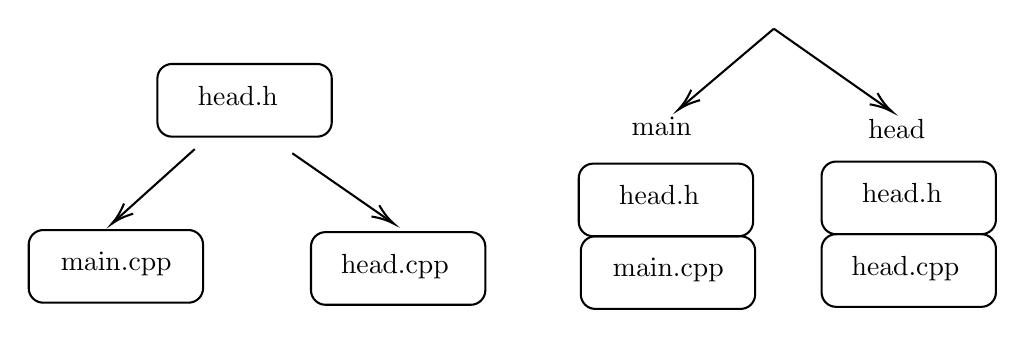
\begin{tikzpicture}[x=0.75pt,y=0.75pt,yscale=-1,xscale=1]
	%uncomment if require: \path (0,300); %set diagram left start at 0, and has height of 300
	
	%Rounded Rect [id:dp8046212658933671] 
	\draw   (119,83) .. controls (119,79.13) and (122.13,76) .. (126,76) -- (196,76) .. controls (199.87,76) and (203,79.13) .. (203,83) -- (203,104) .. controls (203,107.87) and (199.87,111) .. (196,111) -- (126,111) .. controls (122.13,111) and (119,107.87) .. (119,104) -- cycle ;
	%Rounded Rect [id:dp4131717476038639] 
	\draw   (57,163) .. controls (57,159.13) and (60.13,156) .. (64,156) -- (134,156) .. controls (137.87,156) and (141,159.13) .. (141,163) -- (141,184) .. controls (141,187.87) and (137.87,191) .. (134,191) -- (64,191) .. controls (60.13,191) and (57,187.87) .. (57,184) -- cycle ;
	%Rounded Rect [id:dp6275602235598181] 
	\draw   (193,164) .. controls (193,160.13) and (196.13,157) .. (200,157) -- (270,157) .. controls (273.87,157) and (277,160.13) .. (277,164) -- (277,185) .. controls (277,188.87) and (273.87,192) .. (270,192) -- (200,192) .. controls (196.13,192) and (193,188.87) .. (193,185) -- cycle ;
	%Straight Lines [id:da29892507643017163] 
	\draw    (137,117) -- (98.49,151.66) ;
	\draw [shift={(97,153)}, rotate = 318.01] [color={rgb, 255:red, 0; green, 0; blue, 0 }  ][line width=0.75]    (10.93,-3.29) .. controls (6.95,-1.4) and (3.31,-0.3) .. (0,0) .. controls (3.31,0.3) and (6.95,1.4) .. (10.93,3.29)   ;
	%Straight Lines [id:da7604434249637251] 
	\draw    (184,119) -- (231.36,151.86) ;
	\draw [shift={(233,153)}, rotate = 214.76] [color={rgb, 255:red, 0; green, 0; blue, 0 }  ][line width=0.75]    (10.93,-3.29) .. controls (6.95,-1.4) and (3.31,-0.3) .. (0,0) .. controls (3.31,0.3) and (6.95,1.4) .. (10.93,3.29)   ;
	%Rounded Rect [id:dp8118464469584348] 
	\draw   (439,165) .. controls (439,161.13) and (442.13,158) .. (446,158) -- (516,158) .. controls (519.87,158) and (523,161.13) .. (523,165) -- (523,186) .. controls (523,189.87) and (519.87,193) .. (516,193) -- (446,193) .. controls (442.13,193) and (439,189.87) .. (439,186) -- cycle ;
	%Rounded Rect [id:dp6893102005714937] 
	\draw   (323,166) .. controls (323,162.13) and (326.13,159) .. (330,159) -- (400,159) .. controls (403.87,159) and (407,162.13) .. (407,166) -- (407,187) .. controls (407,190.87) and (403.87,194) .. (400,194) -- (330,194) .. controls (326.13,194) and (323,190.87) .. (323,187) -- cycle ;
	%Rounded Rect [id:dp2970948370150095] 
	\draw   (322,131) .. controls (322,127.13) and (325.13,124) .. (329,124) -- (399,124) .. controls (402.87,124) and (406,127.13) .. (406,131) -- (406,152) .. controls (406,155.87) and (402.87,159) .. (399,159) -- (329,159) .. controls (325.13,159) and (322,155.87) .. (322,152) -- cycle ;
	%Rounded Rect [id:dp3048285006841027] 
	\draw   (439,130) .. controls (439,126.13) and (442.13,123) .. (446,123) -- (516,123) .. controls (519.87,123) and (523,126.13) .. (523,130) -- (523,151) .. controls (523,154.87) and (519.87,158) .. (516,158) -- (446,158) .. controls (442.13,158) and (439,154.87) .. (439,151) -- cycle ;
	%Straight Lines [id:da8496668043021236] 
	\draw    (416,59) -- (371.53,96.71) ;
	\draw [shift={(370,98)}, rotate = 319.71] [color={rgb, 255:red, 0; green, 0; blue, 0 }  ][line width=0.75]    (10.93,-3.29) .. controls (6.95,-1.4) and (3.31,-0.3) .. (0,0) .. controls (3.31,0.3) and (6.95,1.4) .. (10.93,3.29)   ;
	%Straight Lines [id:da057864555520047656] 
	\draw    (416,59) -- (471.36,97.85) ;
	\draw [shift={(473,99)}, rotate = 215.06] [color={rgb, 255:red, 0; green, 0; blue, 0 }  ][line width=0.75]    (10.93,-3.29) .. controls (6.95,-1.4) and (3.31,-0.3) .. (0,0) .. controls (3.31,0.3) and (6.95,1.4) .. (10.93,3.29)   ;
	
	% Text Node
	\draw (137,85) node [anchor=north west][inner sep=0.75pt]   [align=left] {head.h};
	% Text Node
	\draw (71,165) node [anchor=north west][inner sep=0.75pt]   [align=left] {main.cpp};
	% Text Node
	\draw (206,166) node [anchor=north west][inner sep=0.75pt]   [align=left] {head.cpp};
	% Text Node
	\draw (452,167) node [anchor=north west][inner sep=0.75pt]   [align=left] {head.cpp};
	% Text Node
	\draw (337,168) node [anchor=north west][inner sep=0.75pt]   [align=left] {main.cpp};
	% Text Node
	\draw (340,133) node [anchor=north west][inner sep=0.75pt]   [align=left] {head.h};
	% Text Node
	\draw (457,132) node [anchor=north west][inner sep=0.75pt]   [align=left] {head.h};
	% Text Node
	\draw (346,100) node [anchor=north west][inner sep=0.75pt]   [align=left] {main};
	% Text Node
	\draw (460,101) node [anchor=north west][inner sep=0.75pt]   [align=left] {head};
	
	
	\end{tikzpicture}
\end{center}

\noindent 每个翻译单元由编译器单独编译, 最终将得到的{\tt .o}文件链接得到可执行文件. 如上图所示程序结构, 在链接时会出现如下问题:

假如在{\tt head.h}文件中定义一个外部链接性变量

\begin{lstlisting}[xleftmargin=2em]
#ifndef HEAD_H
#define HEAD_H
int i = 0;
#endif
\end{lstlisting}
那么在链接时就会出错, 原因是如上两个翻译单元相当于

\begin{center}
	\tikzset{every picture/.style={line width=0.75pt}} %set default line width to 0.75pt        
	
	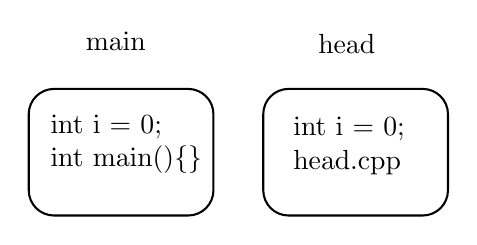
\begin{tikzpicture}[x=0.75pt,y=0.75pt,yscale=-1,xscale=1]
	%uncomment if require: \path (0,300); %set diagram left start at 0, and has height of 300
	
	%Rounded Rect [id:dp31960853174211556] 
	\draw   (225,159.2) .. controls (225,152.46) and (230.46,147) .. (237.2,147) -- (301.8,147) .. controls (308.54,147) and (314,152.46) .. (314,159.2) -- (314,195.8) .. controls (314,202.54) and (308.54,208) .. (301.8,208) -- (237.2,208) .. controls (230.46,208) and (225,202.54) .. (225,195.8) -- cycle ;
	%Rounded Rect [id:dp47295061263468985] 
	\draw   (338,159.2) .. controls (338,152.46) and (343.46,147) .. (350.2,147) -- (414.8,147) .. controls (421.54,147) and (427,152.46) .. (427,159.2) -- (427,195.8) .. controls (427,202.54) and (421.54,208) .. (414.8,208) -- (350.2,208) .. controls (343.46,208) and (338,202.54) .. (338,195.8) -- cycle ;
	
	% Text Node
	\draw (251,118) node [anchor=north west][inner sep=0.75pt]   [align=left] {main};
	% Text Node
	\draw (363,119) node [anchor=north west][inner sep=0.75pt]   [align=left] {head};
	% Text Node
	\draw (234,158) node [anchor=north west][inner sep=0.75pt]   [align=left] {int i = 0;\\int main()\{\}};
	% Text Node
	\draw (351,159.2) node [anchor=north west][inner sep=0.75pt]   [align=left] {int i = 0;\\head.cpp};
	
	
	\end{tikzpicture}
\end{center}

在两个文件中都定义了具有外部链接性的变量i.

\subsubsection{外部链接}
在一个作用域内, 变量能且只能被定义一次, 但是可以被多次声明{\tt( one define rule)}
\begin{paracol}{2}
	\begin{leftcolumn}
		\begin{lstlisting}[title=定义,xleftmargin=2em,xrightmargin=2em]
// 不能在局部作用域内使用
extern int v = 0; 
int v;
		\end{lstlisting}
	\end{leftcolumn}
	\begin{rightcolumn}
		\begin{lstlisting}[title=声明,xleftmargin=2em,xrightmargin=2em]
void func();
extern void func();
extern int v;
		\end{lstlisting}
	\end{rightcolumn}
\end{paracol}

如果需要在多个文件, 指个多翻译单元中使用同一变量, 就必须把定义与声明分离. 变量的定义只能出现在一个文件中, 而在其它用到该变量
	的文件中对其声明.

所以往往头文件中只放一些声明而在另外的文件中进行定义.

\begin{paracol}{2}
	\begin{leftcolumn}
		常见的内部链接类型
		\begin{enumerate}
			\item {\tt const}全局变量
			\item {\tt static}全局变量
			\item {\tt static}函数
			\item {\tt inline}\footnote[1]{{\tt inline} 现在表示在链接时遇到不同编译单元出现了相同签名的函数时只保留一份, 不再是内联的意思.}函数/变量\footnote[2]{{\tt inline variable is C++17 extension}}
			\item 类内定义的成员函数
			\item 类内定义的数据成员(即非静态数据成员)
		\end{enumerate}
	\end{leftcolumn}
	\begin{rightcolumn}
		常见的外部链接类型
		\begin{enumerate}
			\item 全局变量与函数(非{\tt const、static、inline})
			\item 类外定义的数据成员(即静态数据成员在类外的定义)
			\item 类外定义的成员函数
			\item {\tt extern const T v = INIT;}
		\end{enumerate}
	\end{rightcolumn}
\end{paracol}
其它可视为无链接

\vspace{1em}
所有文件中的外部链接性变量会传递给链接器得到一张导出符号表. 记录本编译单元定义, 并且可提供给其它单元
	使用的符号及在本单元对应的地址. 

所有文件中的声明会传递给链接器得到一张未解决符号表, 记录本编译单元有声明但不在本单元定义的符号及其对应的地址, 
	显然在导出符号表中不能存在相同的符号.

\noindent{\tt C11}标准关于{\tt static}和{\tt extern}的内容:
\begin{enumerate}
	\item 若在{\tt extern}声明标识符之前的可见范围内存在对该标识符的声明, 则该标识符的链接与先前声明相同. 
			若无先前声明, 或声明无链接, 则该标识符具有外部链接
	\item 如果在同一翻译单元内, 同一标识符同时出现内外部链接, 则行为未定义
\end{enumerate}
上述原文:

For an identifier declared with the storage-class specifier extern in a scope 
in which a prior declaration of that identifier is visible, if the prior 
declaration specifies internal or external linkage, the linkage of the 
identifier at the later declaration is the same as the linkage specified 
at the prior declaration. If no prior declaration is visible, or if the 
prior declaration specifies no linkage, then the identifier has external 
linkage.

If, within a translation unit, the same identifier appears with both internal 
and external linkage, the behavior is undefined.

\subsubsection{{\tt namespace}中的链接性}
若之前的例子中的全局变量在一个命名空间中, 则不同文件的相同的命名空间中拥有外部链接性.
\columnratio{0.5}
\begin{paracol}{2}
	\begin{leftcolumn}
		\begin{lstlisting}[xleftmargin=6em]
//test1.cpp
int i=2;
					=>
//test2.cpp
extern int i;
		\end{lstlisting}
	\end{leftcolumn}
	\begin{rightcolumn}
		\begin{lstlisting}
//test1.cpp
namespace test{
	int i=2;}
//test2.cpp
namespace test{
	extern int i;}
		\end{lstlisting}
	\end{rightcolumn}
\end{paracol}


\subsection{\color{purple}{{\tt const}关键字}}
\subsubsection{\tt const}
\begin{center}
	\begin{tabular}[b]{|l|l|l|l|}
		\hline
		顶层const&常量指针&int *const ptr&指针本身不能变, 即不能改变指向的对象\\
		\hline
		底层const&指向常量的指针&const int *ptr&不能通过该指针改变指向的对象的内容\\
		\hline
		&常量引用&&引用本身就是一个常量指针\\
		\hline
		底层const&指向常量的引用&const int \&r&相当于指向常量的常量指针\\
		\hline
	\end{tabular}
\end{center}

指向常量的指针或引用都可以绑定到一个常量或者变量上, 当使用指向常量的指针或引用指向一个变量时只表示无法通过该指针去改变该变量值

常量只能绑定到一个指向常量的指针或引用上

\noindent {\tt Note:}
\begin{enumerate}
	\item 顶层{\tt(top-level)const}和底层{\tt(low-level)const}的区别不在于{\tt const}所处的位置
	\item 更一般的, 顶层const可以表示任意的对象是常量, 底层{\tt const}则与指针和引用等复合类型的基本类型部分有关
\end{enumerate}

\begin{lstlisting}[title=三种{\tt const}在开头的顶层{\tt const}]
const int v = 0;//常量指针
constexpr int *p = nullptr;//常量指针, 与cosnt int* p 不同
typedef int* ptr; const ptr p = nullptr;
\end{lstlisting}

\subsubsection{不同场景下的{\tt const}}
\begin{enumerate}
	\item 用于修饰变量, 表明变量是个常量或指向一个常量
	\item 用于修饰函数返回值, 如返回{\tt const}指针, 则只能赋给{\tt const}指针
	\item 用于修饰类内函数{\tt this}指针, 在类内函数尾置{\tt const}
	\begin{itemize}
		\item 表明函数隐式传递的{\tt this}指针是{\tt const this}指针,
				则函数无法改变类内非{\tt mutable}、非{\tt static}、非引用(指针)成员
			 \\ 简单来说, 在{\tt const this}指针视角下, 类内非{\tt mutable}、非{\tt static}
			 	成员都是{\tt const}成员, 并且是顶层{\tt const}, 因此对于类内指针、引用成员, 
				可以改变其指向的值而不能改变其本身
		\item 对于{\tt const}对象, 只能调用尾置{\tt const}成员函数
	\end{itemize}
\end{enumerate}
\subsubsection{\tt constexpr}
常量表达式{\tt (const expression)}是指值不会改变并且在编译过程就能得到计算结果的表达式.

常见的常量表达式有字面值, 用常量表达式初始化的{\tt const}对象.

{\tt constexpr}变量:\quad 用{\tt constexpr}修饰变量, 那么用来初始化这个变量的表达式必须是常量表达式, 否则报错, 其它同{\tt const}

{\tt constexpr}函数:\quad 用{\tt constexpr}修饰函数, 那么只有同时满足
\begin{enumerate}
	\item 所有参数都是常量表达式
	\item 返回的结果被用于常量表达式(比如用于初始化{\tt constexpr}数据)
\end{enumerate}

才会触发编译时求值. 如果只有参数是常量表达式而结果不是, 那么是否触发编译时求值取决于具体实现

\subsection{\color{purple}{其它关键字}}
\subsubsection{\tt explicit}
用于单参数(包括多参数但只有一个参数无默认值)的构造函数首关键字, 表明构造函数不允许从参数类型到类型型的隐式转换
\subsubsection{\tt public protected private}
用于类内:
\begin{enumerate}
	\item {\tt public:} 公有的, 访问不受限制
	\item {\tt protected:} 保护的, 只能在本类、派生类中访问
	\item {\tt private:} 私有的, 只能在本类中访问
\end{enumerate}

用于继承:
\begin{center}
	\begin{tabular}[h]{|c|c|c|c|}
		\hline
		&{\tt public}继承&{\tt protected}继承&{\tt private}继承\\
		\hline
		{\tt public}成员&{\tt public}&\multirow{2}*{\tt protected}&\multirow{2}*{\tt private}\\
		\cline{1-2}
		{\tt protected}成员&{\tt protected}&&\\
		\hline
		{\tt private}成员&\multicolumn{3}{|c|}{不可访问}\\
		\hline
	\end{tabular}
\end{center}
\subsubsection{\tt final <11>}
尾说明符
\begin{itemize}
	\item 用于类, 表明该类禁止被继承
	\item 用于类成员函数, 表明该函数或虚函数禁止被覆盖
\end{itemize}
\subsubsection{\tt override <11>}
尾说明符, 用于标记该虚函数是对基类虚函数的覆盖, 若该函数没有覆盖已存在的虚函数则编译器报错, 用以检查
\subsubsection{\tt friend}
首关键字, 友元函数与友元类, 拥有跟声明所处的类相同的成员访问权限, 不可继承, 因此权限只包括当前类和基类成员
\subsubsection{\tt virtual}
首关键字
\begin{itemize}
	\item 虚继承, 用以解决多继承时命名冲突和冗余数据的问题, 虚继承可以使得在派生类中只保留一份间接基类的成员
	\item 虚函数, 实现动态多态, 派生类重写虚函数不需要加{\tt virtual}, 虚函数{\tt =0}时, 则为纯虚函数, 纯虚函数所在的类称为抽象类
\end{itemize}
\subsubsection{\tt mutable}
\begin{itemize}
	\item 首关键字, 用以修饰类数据成员, 可以使用{\tt const this}指针(尾{\tt const}成员函数)改变{\tt mutable}成员
	\item 尾关键字, 用以表示{\tt lambda}函数展开成仿函数后\sout{重载运算符{\tt ()}函数是非尾{\tt const}成员函数(默认{\tt const}), 
			从而可以改变捕获列表中按值捕获的变量}, 类内成员改为{\tt mutable}成员
\end{itemize}

\subsubsection{\tt volatile}
首关键字
\begin{enumerate}
	\item 声明为{\tt volatile}变量编译器会强制要求读内存, 相关语句不会直接使用上一条语句对应的的寄存器内容
	\item 编译器不会对{\tt volatile}变量进行各种激进的优化,甚至将变量直接消除
	\item 编译器层面上保证{\tt volatile}变量间的顺序性,编译器不会进行乱序优化
	\begin{itemize}
		\item {\tt CPU}依旧有可能乱序执行, 不同于{\tt java}
	\end{itemize}
\end{enumerate}

\subsubsection{\tt typename}
\begin{itemize}
	\item 用于声明模板, 同{\tt class}
	\item 用于表明嵌套从属名称是一个类型
\end{itemize}
\subsubsection{\tt new/delete}

\begin{itemize}
	\item 从自由存储区(考虑{\tt placement new})分配内存, 构造对象, 返回类类型指针
	\item 析构对象, 从堆上释放内存
\end{itemize}

\subsubsection{\tt noexcept <11>}
尾关键字

表明函数不抛出异常
\subsubsection{\tt inline}
表示在链接时遇到不同编译单元出现了相同签名的函数或变量时只保留一份, 不再是内联的意思
\subsubsection{\tt cast <11>}
\begin{itemize}
	\item {\tt static\_cast}用于基本类型转换
	\item {\tt const\_cast}删除变量的{\tt const}属性
	\item {\tt dynamic\_cast}用于将一个父类对象的指针转换为子类对象的指针或引用
	\item {\tt reinterpret\_cast}将一种类型转换为另一种完全不同的类型
\end{itemize}

\subsubsection{\tt extern "C"}
表示之后的代码按照{\tt C}语言的规则去编译

\subsection{\color{purple}{内存布局}}
\begin{figure}[htbp]
	\centering
	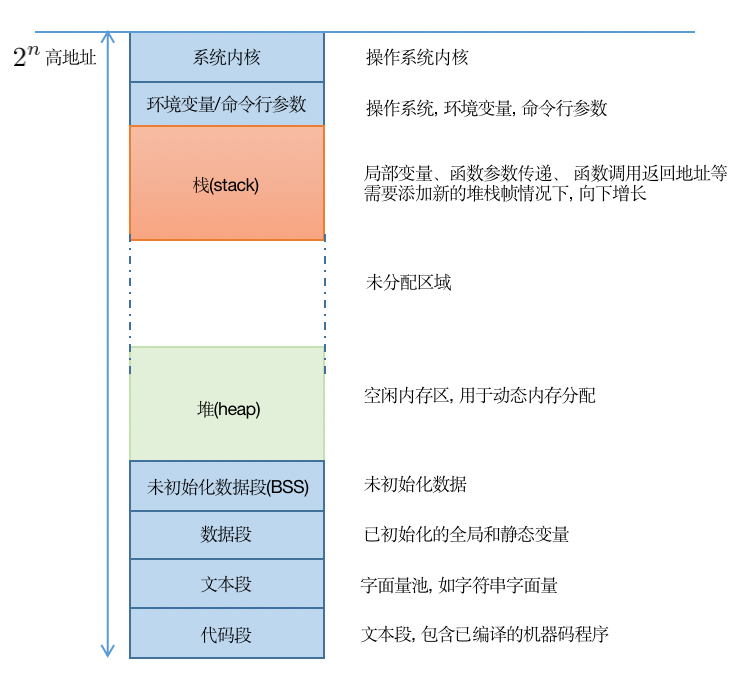
\includegraphics[scale=0.7]{tex_include/pic_include/cpp_basic_memo.png}
\end{figure}

\subsection{\color{purple}{内存分配}}
\subsubsection{概览}
\begin{center}
	\begin{tabular}[h]{|c|c|c|c|c|}
		\hline
		~&{\tt new}&{\tt placement new}&{\tt operator new}&{\tt malloc}\\
		\hline
		性质&关键字&{\tt new}的另一种形式&\multicolumn{2}{|c|}{函数}\\
		\hline
		过程&\makecell[c]{1.分配内存\\2.构造对象\\3.返回对象类型指针}&
			\makecell[c]{1.构造对象\\2.返回对象类型指针}&\multicolumn{2}{|c|}{分配内存}\\
		\hline
		返回类型&\multicolumn{2}{|c|}{类类型指针}&\multicolumn{2}{|c|}{{\tt void*}指针}\\
		\hline
		内存区域&取决于{\tt operator new}&
			\makecell[c]{自由存储区域\\(堆栈、全局、常量等)}&\makecell[c]{一般底层是通过{\tt malloc}\\分配内存在堆上}&堆上\\
		\hline
		重载&\multicolumn{2}{|c|}{不可以重载}&可以重载&\\
		\hline
		失败返回&\multicolumn{2}{|c|}{抛出{\tt bad\_alloc}异常}& &返回{\tt null}\\
		\hline
	\end{tabular}
\end{center}
\begin{lstlisting}[title=三种创建堆上对象方法]
struct obj{ 
	obj(int i):n(i){}
	int n;
};
//1.new
obj* p = new obj(1);

//2.malloc+placement new
void* buf = malloc(sizeof(obj));
obj* p = new(buf) obj(1);

//3.operator new+placement new
void* buf = ::operator new(sizeof(obj));//等于malloc
obj* p = new(buf) obj(1);               //等于手动调用构造函数
\end{lstlisting}
\subsubsection{\tt new/delete and malloc/free}

使用new或delete表达式的过程
\begin{enumerate}
	\item {\tt new}
	\begin{enumerate}
		\item 调用{\tt operator new(}或{\tt operator new[])}函数, 获取一块原始内存, 
			底层可以且一般是{\tt malloc}
		\item 编译器运行相应的构造函数构初始化对象
		\item 返回指向该对象的对象类型指针
	\end{enumerate}
	\item {\tt delete}
	\begin{enumerate}
		\item 对指针指向的对象调用析构函数
		\item 调用{\tt operator delete(}或{\tt operator delete[])}函数释放内存空间, 底层可以且一般是{\tt free}
	\end{enumerate}
\end{enumerate}
\subsubsection{\tt placement new}
{\tt new}表达式分为两种, {\tt new}和{\tt placement new}, 两种表达式的区别在于会调用不同的{\tt operator new}函数
\begin{lstlisting}
	1: new
	obj* p = new obj;
	void* operator new(size_t);
	= operator new(sizeof(obj))
\end{lstlisting}
当使用{\tt new}表达式时, 会自动通过{\tt sizeof}在编译期获得类型大小, 并传递其作为其参数给{\tt operator new}函数
\begin{lstlisting}
	2: placement new
	obj* p = new(address) obj;
	void* operator new(size_t, void*); 
\end{lstlisting}

通过示例中的形式输入一个地址, 会调用这个特殊的两参数的{\tt operator new}函数, \uline{这个函数不可重载}

这个函数接受一个额外的指针(地址), 指向一个已分配好的内存块, 然后直接进行{\tt new}表达式的第二步, 构造对象, 
	并返回指向这个内存块的指针, 其意义相当于手动调用构造函数

{\tt placement new}的地址, 即它指向的内存块不一定要在堆上, 因此一般来说, {\tt new}表达式从自由存储区{\tt (free store)}上为对象动态分配内存空间,
	如通过下面代码将一个对象通过{\tt new}放在栈上

\begin{lstlisting}
class obj{
public:
	obj(int i):n(i){}
	int n;
};
int main(){
	int add; // add所在位置即已分配栈内存
	obj* p = new(&add) obj(3);
	//&add = p
}
\end{lstlisting}
这种{\tt new}出来的对象不能像普通堆对象那样使用{\tt delete}


\subsubsection{{\tt new}重载}

\begin{itemize}
	\item 重载{\tt new/delete}是指重载{\tt operator new}函数而不是重载{\tt new}表达式, 因为{\tt new}本质是一个关键字而不是运算符
	\item 重载{\tt operator new}的意义是不使用默认的内存分配实现(如{\tt malloc}), 自定义内存分配器
	\item {\tt placement new}调用的那个版本的{\tt operator new}函数不能重载
	\item 对于重载{\tt operator new}函数必须定义于类作用域或全局作用域中
	\item 因为{\tt operator new}用于对象构造前, 
			{\tt operator delete}用于对象析构后, 函数与对象无关, 如果位于类作用域即
			在类内重载{\tt operator new}那么它是隐式{\tt static}的, 
			因此类内重载的{\tt operator new/delete}无法访问类内非{\tt static}成员
	\item 可以通过{\tt::operator new}来调用全局的默认的{\tt operator new}函数
\end{itemize}
\subsubsection{{\tt malloc}返回地址}
malloc返回的申请内存的首地址之前, 用额外的字节存储了长度, 即内存块实际首地址不是返回地址
\begin{figure}[htbp]
	\centering
	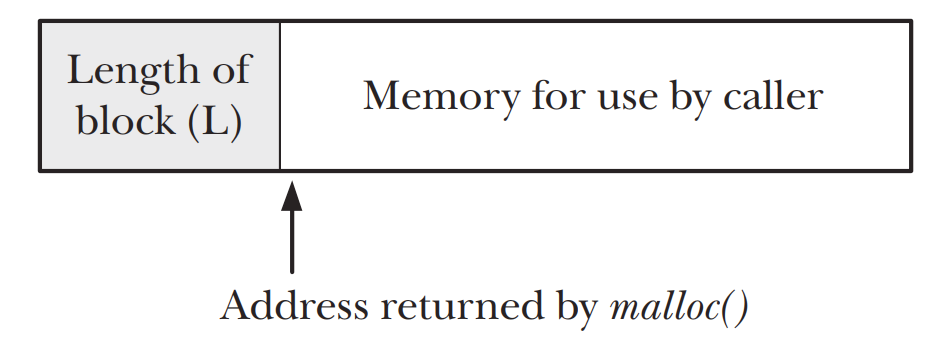
\includegraphics[scale=0.25]{tex_include/pic_include/cpp_basic_malloc.png}
\end{figure}
\subsection{\color{purple}{指针与引用}}
\subsubsection{指针与引用的区别}
\begin{enumerate}
	\item 引用就是常量指针
	\item 引用必须初始化, 且不能改变指向
	\item 无法对引用进行取地址, 或者说只能取到引用指向的对象的地址
	\item 引用的解引用操作由编译器自动进行
\end{enumerate}
\subsubsection{\tt{void*}指针}
指针一般有三个含义
\begin{enumerate}
	\item 指明数据的位置, 体现在指针的值
	\item 表示数据的大小, 例如{\tt int}指针表示四个字节为一组的数据, 体现在指针的步长、自身的加减法计算
	\item 表示数据如何被解释, 例如{\tt float}和{\tt int}都是四字节, 但解释结果完全不同, 体现在指针解引用的结果
\end{enumerate}

{\tt void*} 指针为第一种, 只指明了数据的位置. 以{\tt void*}的视角来看内存空间也仅仅是内存空间, 没办法访问内存空间中所存的对象

对于{\tt void*}类型指针与其它类型指针的转换, {\tt C++}有如下两个规定
\begin{enumerate}
	\item 不允许从{\tt void*}类型到其它类型的隐式转换, 允许从其它类型到{\tt void*}类型的隐式转换, 常见于函数传参
	\item 字面量0可以隐式转换成任意类型的空指针常量
\end{enumerate}

\subsubsection{\tt{nullptr\quad <11>}}

在{\tt C}中, 常用{\tt NULL}来表示空指针
\begin{lstlisting}[xleftmargin=2em]
#define NULL ((void*)0)
\end{lstlisting}
然而在{\tt C++}中不允许从{\tt void*}隐式转换成其它类型的指针, 所以定义了一种新的指针类型, 指针空值类型{\tt std::nullptr\_t}
	, {\tt nullptr}是它的一个实例, 当对指针进行初始化时:
\begin{lstlisting}[xleftmargin=2em]
int *p = nullptr;
int *p = 0;
\end{lstlisting}
两者之间没有区别

\noindent 但在重载情况下:
\begin{lstlisting}[xleftmargin=2em]
void func(int n);
void func(int *p);
\end{lstlisting}
{\tt nullptr}会匹配第二个, 而0实际上两个都能匹配, 在本实验环境中, 会匹配第一项且没有二义性问题

\noindent 若再定义一个
\begin{lstlisting}[xleftmargin=2em]
void func(char *p);
\end{lstlisting}
则{\tt nullptr}会出现二义性错误

至于空指针具体指向哪个地址由编译器管理, 可能是内存中的0号地址, 即指针数据全是0, 也有可能不是

%Effective Modern C++ 第8款, 使用nullptr 而非0, NULL.\\

\subsubsection{野指针}

{\tt wild pointer}也叫悬挂指针, {\tt dangling pointer}

有三种情况会造成野指针:
\begin{enumerate}
	\item 指针未初始化
	\item 指针指向的对象生命周期结束, 如将一个函数体内的局部变量地址传递给外部指针
	\item 指针释放
\end{enumerate}

当指针被{\tt delete}之后, 指针值变为无效, 继续对该指针进行操作会出现{\tt heap use after free}错误.

事实上, 当一个指针被{\tt delete}之后, 指针指向的堆地址空间被释放, 随时可以被分配给其它对象, 但在不同的机器上会有不同的结果.

\noindent 几种特殊情况, 指{\tt delete}之后继续使用指针不报错的情况:
\begin{enumerate}
	\item 指针的数据, 即它指向的地址发生改变, 对它进行解引用会得到0
	\item 地址不改变, 解引用会得到0
	\item 地址不改变, 该内存地址的值也未被擦除, 解引用得到跟{\tt delete}之前一样的结果
\end{enumerate}

准确来讲, {\tt delete}的实际意义是将指针指向的内存空间释放, 以便能分配给其它对象, 但指针本身是否依旧指向那块内存, 
	那块内存的数据是否被擦除未定义

给野指针赋{\tt nullptr}初值避免麻烦

\subsubsection{指向引用的指针, 指向指针的引用}
对引用地址的获取行为会得到引用指向的对象的地址

测试程序见 \href{https://github.com/wenqingqian/Obtuse/blob/main/test/cpp/basic/pointer_reference.cpp}{\tt pointer\_reference}

\begin{center}


	\tikzset{every picture/.style={line width=0.75pt}} %set default line width to 0.75pt        

	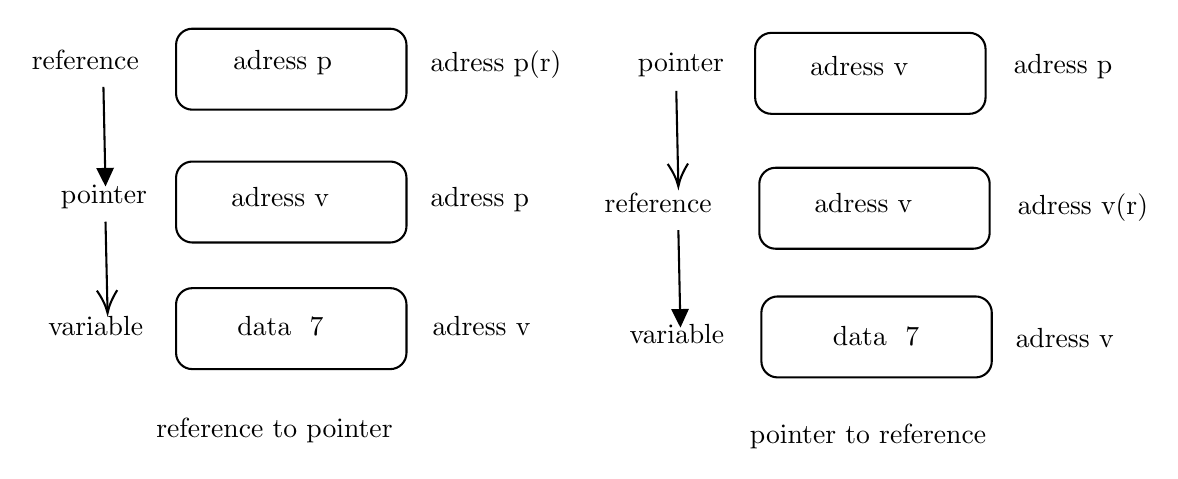
\begin{tikzpicture}[x=0.75pt,y=0.75pt,yscale=-1,xscale=1]
	%uncomment if require: \path (0,300); %set diagram left start at 0, and has height of 300
	
	%Rounded Rect [id:dp11927883071932444] 
	\draw   (85,185.8) .. controls (85,181.49) and (88.49,178) .. (92.8,178) -- (188.2,178) .. controls (192.51,178) and (196,181.49) .. (196,185.8) -- (196,209.2) .. controls (196,213.51) and (192.51,217) .. (188.2,217) -- (92.8,217) .. controls (88.49,217) and (85,213.51) .. (85,209.2) -- cycle ;
	%Rounded Rect [id:dp6640212087116251] 
	\draw   (85,124.8) .. controls (85,120.49) and (88.49,117) .. (92.8,117) -- (188.2,117) .. controls (192.51,117) and (196,120.49) .. (196,124.8) -- (196,148.2) .. controls (196,152.51) and (192.51,156) .. (188.2,156) -- (92.8,156) .. controls (88.49,156) and (85,152.51) .. (85,148.2) -- cycle ;
	%Rounded Rect [id:dp3237041947663375] 
	\draw   (85,60.8) .. controls (85,56.49) and (88.49,53) .. (92.8,53) -- (188.2,53) .. controls (192.51,53) and (196,56.49) .. (196,60.8) -- (196,84.2) .. controls (196,88.51) and (192.51,92) .. (188.2,92) -- (92.8,92) .. controls (88.49,92) and (85,88.51) .. (85,84.2) -- cycle ;
	%Rounded Rect [id:dp9477857736296029] 
	\draw   (367,189.8) .. controls (367,185.49) and (370.49,182) .. (374.8,182) -- (470.2,182) .. controls (474.51,182) and (478,185.49) .. (478,189.8) -- (478,213.2) .. controls (478,217.51) and (474.51,221) .. (470.2,221) -- (374.8,221) .. controls (370.49,221) and (367,217.51) .. (367,213.2) -- cycle ;
	%Rounded Rect [id:dp4721875816932608] 
	\draw   (366,127.8) .. controls (366,123.49) and (369.49,120) .. (373.8,120) -- (469.2,120) .. controls (473.51,120) and (477,123.49) .. (477,127.8) -- (477,151.2) .. controls (477,155.51) and (473.51,159) .. (469.2,159) -- (373.8,159) .. controls (369.49,159) and (366,155.51) .. (366,151.2) -- cycle ;
	%Rounded Rect [id:dp34593900558257906] 
	\draw   (364,62.8) .. controls (364,58.49) and (367.49,55) .. (371.8,55) -- (467.2,55) .. controls (471.51,55) and (475,58.49) .. (475,62.8) -- (475,86.2) .. controls (475,90.51) and (471.51,94) .. (467.2,94) -- (371.8,94) .. controls (367.49,94) and (364,90.51) .. (364,86.2) -- cycle ;
	%Straight Lines [id:da5154723980908134] 
	\draw    (51,146) -- (51.95,188) ;
	\draw [shift={(52,190)}, rotate = 268.7] [color={rgb, 255:red, 0; green, 0; blue, 0 }  ][line width=0.75]    (10.93,-4.9) .. controls (6.95,-2.3) and (3.31,-0.67) .. (0,0) .. controls (3.31,0.67) and (6.95,2.3) .. (10.93,4.9)   ;
	%Straight Lines [id:da5246033953497637] 
	\draw    (50,81) -- (50.94,126) ;
	\draw [shift={(51,129)}, rotate = 268.81] [fill={rgb, 255:red, 0; green, 0; blue, 0 }  ][line width=0.08]  [draw opacity=0] (8.93,-4.29) -- (0,0) -- (8.93,4.29) -- cycle    ;
	%Straight Lines [id:da36423552536908654] 
	\draw    (327,150) -- (327.94,194) ;
	\draw [shift={(328,197)}, rotate = 268.78] [fill={rgb, 255:red, 0; green, 0; blue, 0 }  ][line width=0.08]  [draw opacity=0] (8.93,-4.29) -- (0,0) -- (8.93,4.29) -- cycle    ;
	%Straight Lines [id:da2981001586744325] 
	\draw    (326,83) -- (326.96,127) ;
	\draw [shift={(327,129)}, rotate = 268.75] [color={rgb, 255:red, 0; green, 0; blue, 0 }  ][line width=0.75]    (10.93,-4.9) .. controls (6.95,-2.3) and (3.31,-0.67) .. (0,0) .. controls (3.31,0.67) and (6.95,2.3) .. (10.93,4.9)   ;
	
	% Text Node
	\draw (74,239) node [anchor=north west][inner sep=0.75pt]   [align=left] {reference to pointer};
	% Text Node
	\draw (360,242) node [anchor=north west][inner sep=0.75pt]   [align=left] {pointer to reference};
	% Text Node
	\draw (113,190) node [anchor=north west][inner sep=0.75pt]   [align=left] {data \ 7};
	% Text Node
	\draw (22,190) node [anchor=north west][inner sep=0.75pt]   [align=left] {variable};
	% Text Node
	\draw (207,190) node [anchor=north west][inner sep=0.75pt]   [align=left] {adress v};
	% Text Node
	\draw (28,127) node [anchor=north west][inner sep=0.75pt]   [align=left] {pointer};
	% Text Node
	\draw (206,128) node [anchor=north west][inner sep=0.75pt]   [align=left] {adress p};
	% Text Node
	\draw (14,62) node [anchor=north west][inner sep=0.75pt]   [align=left] {reference};
	% Text Node
	\draw (206,62) node [anchor=north west][inner sep=0.75pt]   [align=left] {adress p(r)};
	% Text Node
	\draw (111,62) node [anchor=north west][inner sep=0.75pt]   [align=left] {adress p};
	% Text Node
	\draw (110,128) node [anchor=north west][inner sep=0.75pt]   [align=left] {adress v};
	% Text Node
	\draw (290,131) node [anchor=north west][inner sep=0.75pt]   [align=left] {reference};
	% Text Node
	\draw (306,63) node [anchor=north west][inner sep=0.75pt]   [align=left] {pointer};
	% Text Node
	\draw (302,194) node [anchor=north west][inner sep=0.75pt]   [align=left] {variable};
	% Text Node
	\draw (488,196) node [anchor=north west][inner sep=0.75pt]   [align=left] {adress v};
	% Text Node
	\draw (400,195) node [anchor=north west][inner sep=0.75pt]   [align=left] {data \ 7};
	% Text Node
	\draw (487,64) node [anchor=north west][inner sep=0.75pt]   [align=left] {adress p};
	% Text Node
	\draw (489,131) node [anchor=north west][inner sep=0.75pt]   [align=left] {adress v(r)};
	% Text Node
	\draw (391,131) node [anchor=north west][inner sep=0.75pt]   [align=left] {adress v};
	% Text Node
	\draw (389,65) node [anchor=north west][inner sep=0.75pt]   [align=left] {adress v};
	
	
	\end{tikzpicture}
\end{center}


%------------------------------------------------------------------------------------------------%
%-------------------------------------Section object-oriented---------------------------%
%------------------------------------------------------------------------------------------------%
\begin{comment}
\section{\color{blue}{面向对象}}

\subsection{\color{purple}{多态的实现原理和应用场景}}
%------------------------------------------------------------------------------------------------%
%-------------------------------------Section STL---------------------------------------%
%------------------------------------------------------------------------------------------------%
\section{\color{blue}{\tt STL}}

\subsection{\color{purple}{线程安全的实现及标准容器库的线程安全性}}
\subsection{\color{purple}{{\tt sort}算法是怎么实现的}}
\end{comment}
%------------------------------------------------------------------------------------------------%
%-------------------------------------Section C++11------------------------------------%
\section{\color{blue}{\tt C++11}}

\subsection{\color{purple}{\tt{decltype}和\tt{auto}}}

\columnratio{0.5}
\begin{paracol}{2}
	\begin{leftcolumn}
		\begin{lstlisting}[title=decltype,basicstyle=\small,columns=flexible,xleftmargin=1em,xrightmargin=1em]
int *r=0;
decltype (*r+0) a;//表达式结果为int, 因此a为int
decltype (r) a;//a是指针
decltype (*r) a = ini;//a是引用
decltype ((r)) a = ini;//a是指向指针的引用
decltype ((*r)) a = ini;//a是引用 
		\end{lstlisting}
		{\tt decltype((variable))}的结果永远是引用.
	\end{leftcolumn}
	\begin{rightcolumn}
		\uline{{\tt auto}一般会忽略顶层{\tt const}, 保留底层{\tt const}}, 引用本身就是一个顶层{\tt const}指针, 因此{\tt auto}类型推导不会直接得到引用类型
		\begin{lstlisting}[basicstyle=\small,columns=flexible,xleftmargin=2em,xrightmargin=2em]
const int i = 1; const int&r = i;
auto a = i;//a是int
auto a = &i;//a是const int*(底层const)
auto a = r;//a是int
auto &a = i;//a是左引用
auto &&a;(万能引用)
		\end{lstlisting}
	\end{rightcolumn}
\end{paracol}
\subsection{\color{purple}{左右值}}
\subsubsection{左值与右值}
 \href{https://zhuanlan.zhihu.com/p/402251966}{原文}

左值是一个对象, 可以用\&取地址, 而右值更贴近“值”本身. 一般来说, 表达式结束后, 
	值是否有\uline{显式}的存储位置是左右值的区分(右值可以隐式存在内存中)

\columnratio{0.5}
\begin{paracol}{2}
	\begin{leftcolumn}
		左值:
		\begin{enumerate}
			\item 字符串字面量
			\item 内置的前{\tt ++}与前{\tt --}
			\item 右值引用类型变量
			\item 转型为左值引用的表达式
			\item *解引用的表达式
		\end{enumerate}
	\end{leftcolumn}
	\begin{rightcolumn}
		右值:
		\begin{enumerate}
			\item 非字符串的字面量以及枚举项
			\item 置的后{\tt++}与后{\tt- -}
			\item 内置的算术, 逻辑, 比较表达式
			\item 内置取地址表达式, {\tt this}指针
			\item 未命名的{\tt lambda}表达式
			\item 转型为非引用的表达式
			\item 转型为右值引用的表达式
		\end{enumerate}
	\end{rightcolumn}
\end{paracol}
\subsubsection{左值引用与右值引用}

左右值并不是{\tt C++11}才有的新概念, 而右值引用是{\tt C++11}为了处理
	无需深拷贝的资源转移型需求而引入

左右引用只能处理对应的左右值. 一个例外是{\tt const T\&}, 既可以引用左值, 也可以引用右值

\noindent 即可以写出这样的代码
\begin{lstlisting}[basicstyle=\small,columns=flexible,xleftmargin=14em]
const int& clr = 1; const int& clr2 = clr;
\end{lstlisting}

\vspace*{2em}
\columnratio{0.4}
\begin{paracol}{2}
	\begin{leftcolumn}
		对于右值来说, 不能真正取地址, 而引用实质就是操作地址指针, 因此理论上无法进行左引用. 对于左值来说, 
			可以显式转换成右值引用

		如右值例7, 转换为右值引用的表达式本身是一个右值, 但是通过右值引用绑定到的对象自身是一个左值, 即左值例3
	\end{leftcolumn}
	\begin{rightcolumn}
		\begin{lstlisting}[basicstyle=\small,columns=flexible,xleftmargin=5em,xrightmargin=5em]
//可以将左值转为右值, 再进行右引用
Test t(1);
// 使用std::move转为右值引用
Test&& t1 = std::move(t);
// 使用static_cast转为右值引用
Test&& t2 = static_cast<Test&&>(t);
// 使用C风格强转为右值引用
Test&& t3 = (Test&&)t;
// 使用std::forwad<T&&>为右值引用
Test&& t4 = std::forward<T&&>(t);
		\end{lstlisting}
	\end{rightcolumn}
\end{paracol}
\subsection{\color{purple}{移动语义与完美转发}}
\subsubsection{浅拷贝与深拷贝}
\columnratio{0.5}
\begin{paracol}{2}
	
	\begin{leftcolumn}
	当通过一个对象初始化另一个对象时,

	如 \uline{{\tt Test a(10);}}\uline{{\tt Test b(a);}}时:

	假设{\tt Test}中有资源拖管
		
	只记录资源{\tt Data}的指针, 而非记录资源全部信息到类对象里面, 
		构造时从堆上用{\tt new}申请内存供资源后面使用, 析构时从堆上释放内存, 回收掉资源, 
		中间过程资源读写操作都通过指针{\tt p}来完成. {\tt C++}对象构造与析构函数的成对调用, 
		也保证了安全性与不发生泄露({\tt RAII})
	\end{leftcolumn}
	\begin{rightcolumn}
\begin{lstlisting}[xleftmargin=2em,xrightmargin=2em]
class Test1 public:
	Test1(int s):size(s) 
		p = new char[size];
	~Test1()
		if(p)  delete []p; 
			   p = nullptr;
	int size;
	char* p;
\end{lstlisting}	
	\end{rightcolumn}
\end{paracol}

以右侧结构为例: 

\begin{center}




	\tikzset{every picture/.style={line width=0.75pt}} %set default line width to 0.75pt        

	\begin{tikzpicture}[x=0.75pt,y=0.75pt,yscale=-1,xscale=1]
	%uncomment if require: \path (0,246); %set diagram left start at 0, and has height of 246
	
	%Rounded Rect [id:dp9814564185052337] 
	\draw   (144.09,96.49) .. controls (144.09,92.04) and (147.7,88.43) .. (152.15,88.43) -- (198.94,88.43) .. controls (203.39,88.43) and (207,92.04) .. (207,96.49) -- (207,120.68) .. controls (207,125.13) and (203.39,128.74) .. (198.94,128.74) -- (152.15,128.74) .. controls (147.7,128.74) and (144.09,125.13) .. (144.09,120.68) -- cycle ;
	%Rounded Rect [id:dp13504310460610203] 
	\draw   (3,96.49) .. controls (3,92.04) and (6.61,88.43) .. (11.06,88.43) -- (57.85,88.43) .. controls (62.3,88.43) and (65.91,92.04) .. (65.91,96.49) -- (65.91,120.68) .. controls (65.91,125.13) and (62.3,128.74) .. (57.85,128.74) -- (11.06,128.74) .. controls (6.61,128.74) and (3,125.13) .. (3,120.68) -- cycle ;
	%Shape: Ellipse [id:dp35837246392687105] 
	\draw   (11.99,170.01) .. controls (11.99,156.76) and (22.05,146.01) .. (34.45,146.01) .. controls (46.86,146.01) and (56.92,156.76) .. (56.92,170.01) .. controls (56.92,183.26) and (46.86,194) .. (34.45,194) .. controls (22.05,194) and (11.99,183.26) .. (11.99,170.01) -- cycle ;
	%Rounded Rect [id:dp20403462657508187] 
	\draw   (362.7,96.38) .. controls (362.7,91.97) and (366.28,88.39) .. (370.69,88.39) -- (421.01,88.39) .. controls (425.42,88.39) and (429,91.97) .. (429,96.38) -- (429,120.34) .. controls (429,124.75) and (425.42,128.33) .. (421.01,128.33) -- (370.69,128.33) .. controls (366.28,128.33) and (362.7,124.75) .. (362.7,120.34) -- cycle ;
	%Rounded Rect [id:dp7768537420240913] 
	\draw   (214,96.38) .. controls (214,91.97) and (217.58,88.39) .. (221.99,88.39) -- (272.31,88.39) .. controls (276.72,88.39) and (280.3,91.97) .. (280.3,96.38) -- (280.3,120.34) .. controls (280.3,124.75) and (276.72,128.33) .. (272.31,128.33) -- (221.99,128.33) .. controls (217.58,128.33) and (214,124.75) .. (214,120.34) -- cycle ;
	%Shape: Ellipse [id:dp5039225164311434] 
	\draw   (220.47,171.22) .. controls (220.47,158.09) and (231.07,147.45) .. (244.15,147.45) .. controls (257.23,147.45) and (267.83,158.09) .. (267.83,171.22) .. controls (267.83,184.36) and (257.23,195) .. (244.15,195) .. controls (231.07,195) and (220.47,184.36) .. (220.47,171.22) -- cycle ;
	%Shape: Ellipse [id:dp3337480641475472] 
	\draw   (371.17,170.32) .. controls (371.17,157.19) and (381.77,146.55) .. (394.85,146.55) .. controls (407.93,146.55) and (418.53,157.19) .. (418.53,170.32) .. controls (418.53,183.45) and (407.93,194.1) .. (394.85,194.1) .. controls (381.77,194.1) and (371.17,183.45) .. (371.17,170.32) -- cycle ;
	%Rounded Rect [id:dp44340954001106425] 
	\draw   (585.39,96.85) .. controls (585.39,92.61) and (588.83,89.17) .. (593.07,89.17) -- (644.32,89.17) .. controls (648.56,89.17) and (652,92.61) .. (652,96.85) -- (652,119.89) .. controls (652,124.13) and (648.56,127.57) .. (644.32,127.57) -- (593.07,127.57) .. controls (588.83,127.57) and (585.39,124.13) .. (585.39,119.89) -- cycle ;
	%Rounded Rect [id:dp7095396196135548] 
	\draw   (436,96.85) .. controls (436,92.61) and (439.44,89.17) .. (443.68,89.17) -- (494.93,89.17) .. controls (499.17,89.17) and (502.61,92.61) .. (502.61,96.85) -- (502.61,119.89) .. controls (502.61,124.13) and (499.17,127.57) .. (494.93,127.57) -- (443.68,127.57) .. controls (439.44,127.57) and (436,124.13) .. (436,119.89) -- cycle ;
	%Shape: Ellipse [id:dp8281848505805895] 
	\draw   (504.52,167.88) .. controls (504.52,155.25) and (515.17,145.02) .. (528.3,145.02) .. controls (541.44,145.02) and (552.09,155.25) .. (552.09,167.88) .. controls (552.09,180.5) and (541.44,190.73) .. (528.3,190.73) .. controls (515.17,190.73) and (504.52,180.5) .. (504.52,167.88) -- cycle ;
	\draw   (492.61,127.03) -- (489.54,146.53)(500.9,138.32) -- (481.25,135.24) ;
	
	% Text Node
	\draw (84.56,18.13) node [anchor=north west][inner sep=0.75pt]  [font=\normalsize] [align=left] {浅拷贝};
	% Text Node
	\draw (304.76,12.92) node [anchor=north west][inner sep=0.75pt]  [font=\normalsize] [align=left] {深拷贝};
	% Text Node
	\draw (23.56,53.58) node [anchor=north west][inner sep=0.75pt]  [font=\small] [align=left] {old};
	% Text Node
	\draw (161.6,52.62) node [anchor=north west][inner sep=0.75pt]  [font=\small] [align=left] {new};
	% Text Node
	\draw (94.55,48.55) node [anchor=north west][inner sep=0.75pt]  [font=\small,rotate=-359.26] [align=left] {copy};
	% Text Node
	\draw (151.21,91.01) node [anchor=north west][inner sep=0.75pt]  [font=\small] [align=left] {int size};
	% Text Node
	\draw (152.6,109.24) node [anchor=north west][inner sep=0.75pt]  [font=\small] [align=left] {char* p};
	% Text Node
	\draw (10.12,91.01) node [anchor=north west][inner sep=0.75pt]  [font=\small] [align=left] {int size};
	% Text Node
	\draw (9.71,108.28) node [anchor=north west][inner sep=0.75pt]  [font=\small] [align=left] {char* p};
	% Text Node
	\draw (19.43,154.18) node [anchor=north west][inner sep=0.75pt]  [font=\small] [align=left] {new \\char[]};
	% Text Node
	\draw (94.39,84.91) node [anchor=north west][inner sep=0.75pt]  [font=\small,rotate=-359.26] [align=left] {copy};
	% Text Node
	\draw (95.45,103.14) node [anchor=north west][inner sep=0.75pt]  [font=\small,rotate=-359.26] [align=left] {copy};
	% Text Node
	\draw (236.2,53.79) node [anchor=north west][inner sep=0.75pt]  [font=\small] [align=left] {old};
	% Text Node
	\draw (381.88,52.83) node [anchor=north west][inner sep=0.75pt]  [font=\small] [align=left] {new};
	% Text Node
	\draw (311.27,48.8) node [anchor=north west][inner sep=0.75pt]  [font=\small,rotate=-359.26] [align=left] {copy};
	% Text Node
	\draw (371.39,90.87) node [anchor=north west][inner sep=0.75pt]  [font=\small] [align=left] {int size};
	% Text Node
	\draw (372.88,108.94) node [anchor=north west][inner sep=0.75pt]  [font=\small] [align=left] {char* p};
	% Text Node
	\draw (222.69,90.87) node [anchor=north west][inner sep=0.75pt]  [font=\small] [align=left] {int size};
	% Text Node
	\draw (222.28,107.99) node [anchor=north west][inner sep=0.75pt]  [font=\small] [align=left] {char* p};
	% Text Node
	\draw (230.15,156.42) node [anchor=north west][inner sep=0.75pt]  [font=\small] [align=left] {new \\char[]};
	% Text Node
	\draw (313.16,86.84) node [anchor=north west][inner sep=0.75pt]  [font=\small,rotate=-359.26] [align=left] {copy};
	% Text Node
	\draw (380.85,153.57) node [anchor=north west][inner sep=0.75pt]  [font=\small] [align=left] {new \\char[]};
	% Text Node
	\draw (313.16,149.61) node [anchor=north west][inner sep=0.75pt]  [font=\small,rotate=-359.26] [align=left] {copy};
	% Text Node
	\draw (523.28,11) node [anchor=north west][inner sep=0.75pt]  [font=\normalsize] [align=left] {移动语义};
	% Text Node
	\draw (458.35,55.62) node [anchor=north west][inner sep=0.75pt]  [font=\small] [align=left] {old};
	% Text Node
	\draw (604.72,54.71) node [anchor=north west][inner sep=0.75pt]  [font=\small] [align=left] {new};
	% Text Node
	\draw (533.78,50.87) node [anchor=north west][inner sep=0.75pt]  [font=\small,rotate=-359.26] [align=left] {move};
	% Text Node
	\draw (594.22,91.27) node [anchor=north west][inner sep=0.75pt]  [font=\small] [align=left] {int size};
	% Text Node
	\draw (595.72,108.64) node [anchor=north west][inner sep=0.75pt]  [font=\small] [align=left] {char* p};
	% Text Node
	\draw (444.83,91.27) node [anchor=north west][inner sep=0.75pt]  [font=\small] [align=left] {int size};
	% Text Node
	\draw (444.43,107.73) node [anchor=north west][inner sep=0.75pt]  [font=\small] [align=left] {char* p};
	% Text Node
	\draw (513.3,152.22) node [anchor=north west][inner sep=0.75pt]  [font=\small] [align=left] {new \\char[]};
	% Text Node
	\draw (535.69,87.44) node [anchor=north west][inner sep=0.75pt]  [font=\small,rotate=-359.26] [align=left] {copy};
	% Text Node
	\draw (537.69,102.44) node [anchor=north west][inner sep=0.75pt]  [font=\small,rotate=-359.26] [align=left] {copy};
	% Text Node
	\draw (450,166) node [anchor=north west][inner sep=0.75pt]  [font=\small] [align=left] {{\small nullptr}};
	% Connection
	\draw [color={rgb, 255:red, 175; green, 0; blue, 50 }  ,draw opacity=1 ]   (158.6,60.23) -- (48.56,60.98) ;
	\draw [shift={(46.56,60.99)}, rotate = 359.61] [color={rgb, 255:red, 175; green, 0; blue, 50 }  ,draw opacity=1 ][line width=0.75]    (10.93,-3.29) .. controls (6.95,-1.4) and (3.31,-0.3) .. (0,0) .. controls (3.31,0.3) and (6.95,1.4) .. (10.93,3.29)   ;
	% Connection
	\draw    (174.53,71.62) -- (173.87,85.01) ;
	\draw [shift={(173.78,87.01)}, rotate = 272.81] [color={rgb, 255:red, 0; green, 0; blue, 0 }  ][line width=0.75]    (10.93,-3.29) .. controls (6.95,-1.4) and (3.31,-0.3) .. (0,0) .. controls (3.31,0.3) and (6.95,1.4) .. (10.93,3.29)   ;
	% Connection
	\draw    (33.29,127.28) -- (35.26,148.19) ;
	\draw [shift={(35.45,150.18)}, rotate = 264.61] [color={rgb, 255:red, 0; green, 0; blue, 0 }  ][line width=0.75]    (10.93,-3.29) .. controls (6.95,-1.4) and (3.31,-0.3) .. (0,0) .. controls (3.31,0.3) and (6.95,1.4) .. (10.93,3.29)   ;
	% Connection
	\draw    (33.11,72.58) -- (32.64,85.01) ;
	\draw [shift={(32.56,87.01)}, rotate = 272.2] [color={rgb, 255:red, 0; green, 0; blue, 0 }  ][line width=0.75]    (10.93,-3.29) .. controls (6.95,-1.4) and (3.31,-0.3) .. (0,0) .. controls (3.31,0.3) and (6.95,1.4) .. (10.93,3.29)   ;
	% Connection
	\draw [color={rgb, 255:red, 175; green, 0; blue, 50 }  ,draw opacity=1 ]   (148.21,98.51) -- (59.12,98.51) ;
	\draw [shift={(57.12,98.51)}, rotate = 360] [color={rgb, 255:red, 175; green, 0; blue, 50 }  ,draw opacity=1 ][line width=0.75]    (10.93,-3.29) .. controls (6.95,-1.4) and (3.31,-0.3) .. (0,0) .. controls (3.31,0.3) and (6.95,1.4) .. (10.93,3.29)   ;
	% Connection
	\draw [color={rgb, 255:red, 175; green, 0; blue, 50 }  ,draw opacity=1 ]   (149.6,116.57) -- (59.71,115.97) ;
	\draw [shift={(57.71,115.95)}, rotate = 0.38] [color={rgb, 255:red, 175; green, 0; blue, 50 }  ,draw opacity=1 ][line width=0.75]    (10.93,-3.29) .. controls (6.95,-1.4) and (3.31,-0.3) .. (0,0) .. controls (3.31,0.3) and (6.95,1.4) .. (10.93,3.29)   ;
	% Connection
	\draw [color={rgb, 255:red, 175; green, 0; blue, 50 }  ,draw opacity=1 ]   (149.6,126.83) -- (60.29,162.14) ;
	\draw [shift={(58.43,162.88)}, rotate = 338.42] [color={rgb, 255:red, 175; green, 0; blue, 50 }  ,draw opacity=1 ][line width=0.75]    (10.93,-3.29) .. controls (6.95,-1.4) and (3.31,-0.3) .. (0,0) .. controls (3.31,0.3) and (6.95,1.4) .. (10.93,3.29)   ;
	% Connection
	\draw [color={rgb, 255:red, 175; green, 0; blue, 50 }  ,draw opacity=1 ]   (378.88,60.44) -- (261.2,61.19) ;
	\draw [shift={(259.2,61.2)}, rotate = 359.63] [color={rgb, 255:red, 175; green, 0; blue, 50 }  ,draw opacity=1 ][line width=0.75]    (10.93,-3.29) .. controls (6.95,-1.4) and (3.31,-0.3) .. (0,0) .. controls (3.31,0.3) and (6.95,1.4) .. (10.93,3.29)   ;
	% Connection
	\draw    (394.78,71.83) -- (394.09,84.88) ;
	\draw [shift={(393.99,86.87)}, rotate = 272.99] [color={rgb, 255:red, 0; green, 0; blue, 0 }  ][line width=0.75]    (10.93,-3.29) .. controls (6.95,-1.4) and (3.31,-0.3) .. (0,0) .. controls (3.31,0.3) and (6.95,1.4) .. (10.93,3.29)   ;
	% Connection
	\draw    (245.45,126.99) -- (246.81,150.42) ;
	\draw [shift={(246.93,152.42)}, rotate = 266.67] [color={rgb, 255:red, 0; green, 0; blue, 0 }  ][line width=0.75]    (10.93,-3.29) .. controls (6.95,-1.4) and (3.31,-0.3) .. (0,0) .. controls (3.31,0.3) and (6.95,1.4) .. (10.93,3.29)   ;
	% Connection
	\draw    (245.73,72.79) -- (245.24,84.88) ;
	\draw [shift={(245.16,86.87)}, rotate = 272.34] [color={rgb, 255:red, 0; green, 0; blue, 0 }  ][line width=0.75]    (10.93,-3.29) .. controls (6.95,-1.4) and (3.31,-0.3) .. (0,0) .. controls (3.31,0.3) and (6.95,1.4) .. (10.93,3.29)   ;
	% Connection
	\draw [color={rgb, 255:red, 175; green, 0; blue, 50 }  ,draw opacity=1 ]   (368.39,98.37) -- (271.69,98.37) ;
	\draw [shift={(269.69,98.37)}, rotate = 360] [color={rgb, 255:red, 175; green, 0; blue, 50 }  ,draw opacity=1 ][line width=0.75]    (10.93,-3.29) .. controls (6.95,-1.4) and (3.31,-0.3) .. (0,0) .. controls (3.31,0.3) and (6.95,1.4) .. (10.93,3.29)   ;
	% Connection
	\draw    (396.11,127.94) -- (397.37,147.57) ;
	\draw [shift={(397.5,149.57)}, rotate = 266.33] [color={rgb, 255:red, 0; green, 0; blue, 0 }  ][line width=0.75]    (10.93,-3.29) .. controls (6.95,-1.4) and (3.31,-0.3) .. (0,0) .. controls (3.31,0.3) and (6.95,1.4) .. (10.93,3.29)   ;
	% Connection
	\draw [color={rgb, 255:red, 175; green, 0; blue, 50 }  ,draw opacity=1 ]   (377.85,170.97) -- (271.15,172.99) ;
	\draw [shift={(269.15,173.02)}, rotate = 358.92] [color={rgb, 255:red, 175; green, 0; blue, 50 }  ,draw opacity=1 ][line width=0.75]    (10.93,-3.29) .. controls (6.95,-1.4) and (3.31,-0.3) .. (0,0) .. controls (3.31,0.3) and (6.95,1.4) .. (10.93,3.29)   ;
	% Connection
	\draw [color={rgb, 255:red, 175; green, 0; blue, 50 }  ,draw opacity=1 ]   (601.72,62.31) -- (483.35,63.03) ;
	\draw [shift={(481.35,63.04)}, rotate = 359.65] [color={rgb, 255:red, 175; green, 0; blue, 50 }  ,draw opacity=1 ][line width=0.75]    (10.93,-3.29) .. controls (6.95,-1.4) and (3.31,-0.3) .. (0,0) .. controls (3.31,0.3) and (6.95,1.4) .. (10.93,3.29)   ;
	% Connection
	\draw    (617.59,73.71) -- (616.96,85.28) ;
	\draw [shift={(616.85,87.27)}, rotate = 273.13] [color={rgb, 255:red, 0; green, 0; blue, 0 }  ][line width=0.75]    (10.93,-3.29) .. controls (6.95,-1.4) and (3.31,-0.3) .. (0,0) .. controls (3.31,0.3) and (6.95,1.4) .. (10.93,3.29)   ;
	% Connection
	\draw    (480.64,126.73) -- (508.77,150.32) ;
	\draw [shift={(510.3,151.61)}, rotate = 219.99] [color={rgb, 255:red, 0; green, 0; blue, 0 }  ][line width=0.75]    (10.93,-3.29) .. controls (6.95,-1.4) and (3.31,-0.3) .. (0,0) .. controls (3.31,0.3) and (6.95,1.4) .. (10.93,3.29)   ;
	% Connection
	\draw    (467.86,74.62) -- (467.41,85.27) ;
	\draw [shift={(467.32,87.27)}, rotate = 272.45] [color={rgb, 255:red, 0; green, 0; blue, 0 }  ][line width=0.75]    (10.93,-3.29) .. controls (6.95,-1.4) and (3.31,-0.3) .. (0,0) .. controls (3.31,0.3) and (6.95,1.4) .. (10.93,3.29)   ;
	% Connection
	\draw [color={rgb, 255:red, 175; green, 0; blue, 50 }  ,draw opacity=1 ]   (591.22,98.77) -- (493.83,98.77) ;
	\draw [shift={(491.83,98.77)}, rotate = 360] [color={rgb, 255:red, 175; green, 0; blue, 50 }  ,draw opacity=1 ][line width=0.75]    (10.93,-3.29) .. controls (6.95,-1.4) and (3.31,-0.3) .. (0,0) .. controls (3.31,0.3) and (6.95,1.4) .. (10.93,3.29)   ;
	% Connection
	\draw [color={rgb, 255:red, 175; green, 0; blue, 50 }  ,draw opacity=1 ]   (592.72,115.99) -- (494.43,115.39) ;
	\draw [shift={(492.43,115.38)}, rotate = 0.35] [color={rgb, 255:red, 175; green, 0; blue, 50 }  ,draw opacity=1 ][line width=0.75]    (10.93,-3.29) .. controls (6.95,-1.4) and (3.31,-0.3) .. (0,0) .. controls (3.31,0.3) and (6.95,1.4) .. (10.93,3.29)   ;
	% Connection
	\draw [color={rgb, 255:red, 175; green, 0; blue, 50 }  ,draw opacity=1 ]   (599.39,127.64) -- (554.01,155.35) ;
	\draw [shift={(552.3,156.4)}, rotate = 328.59] [color={rgb, 255:red, 175; green, 0; blue, 50 }  ,draw opacity=1 ][line width=0.75]    (10.93,-3.29) .. controls (6.95,-1.4) and (3.31,-0.3) .. (0,0) .. controls (3.31,0.3) and (6.95,1.4) .. (10.93,3.29)   ;
	% Connection
	\draw    (467.04,126.73) -- (467.37,160) ;
	\draw [shift={(467.39,162)}, rotate = 269.43] [color={rgb, 255:red, 0; green, 0; blue, 0 }  ][line width=0.75]    (10.93,-3.29) .. controls (6.95,-1.4) and (3.31,-0.3) .. (0,0) .. controls (3.31,0.3) and (6.95,1.4) .. (10.93,3.29)   ;
	
	\end{tikzpicture}
\end{center}


\begin{enumerate}
	\item 浅拷贝: 没有真正new内存, 两者共用一块内存地址, 当最后都析构时, 这块内存会被析构两次, 发生crash
	\item 深拷贝: 将指针指向的资源深入复制了一份
	\item 移动语义: 当原对象不再使用, 使用移动语义, 转移资源, 减少拷贝
\end{enumerate}
参考代码见 \href{https://github.com/wenqingqian/Obtuse/blob/main/test/cpp/c++11/copy_move_constructor}{\tt copy\_move\_constructor}
\subsubsection{移动语义}
移动语义: 一个对象的资源在销毁前, 将其转移给其它对象再用起来, 这样能减少资源带来的构造开销, 程序获得更高的效能

移动语义的使用场景就是需要深拷贝原对象的资源, 而原对象不再使用, 就可以使用移动语义, 本质就是在浅拷贝的基础上
	将原对象具有资源的指针置空.

在{\tt C++11}之前, 移动语义使用的问题:
\begin{enumerate}
	\item 使用移动语义需要在构造函数中加额外的参数来选择是否使用移动语义
	\item 因为需要修改类内数据, 无法使用拷贝构造函数({\tt const T\&})
	\item 非{\tt const}引用又无法引用右值, 并且也需要{\tt const}引用来处理{\tt const}对象
\end{enumerate}

{\tt C++11}直接统一, 增加{\tt \&\&}右值引用, 事情变简单, 想要深拷贝的就{\tt T(const T\&)}实现;
	想要移动拷贝的就实现{\tt T(T\&\&)}. 两者都实现时, 一旦传入是个右值, 根据重载机制会优先
	触发移动拷贝构造调用, 使用移动语意, 转移资源, 减少拷贝

{\tt ->}\quad 底层{\tt const}可用于重载而顶层不能, 对于非{\tt const}对象会优先匹配非{\tt const}引用
\subsubsection{万能引用与引用折叠}

对于一个模板
\begin{lstlisting}[xleftmargin=10em,xrightmargin=10em]
template<typename T> T func(T para){}
\end{lstlisting}

\columnratio{0.25}
\begin{paracol}{2}
	\begin{leftcolumn}
		因为引用与引用的对象是没有区别的, 当传入一个引用时, 无法像指针那样分辨出来.
	\end{leftcolumn}
	\begin{rightcolumn}
		\begin{lstlisting}[xleftmargin=1em]
int i = 1; func(i); -- int func<int >(int para){} 
int&r = i; func(r); -- int func<int >(int para){}
int*p =&i; func(p); -- int*func<int*>(int*para){} 
		\end{lstlisting}
	\end{rightcolumn}
	\begin{leftcolumn*}
		所以当需要引用一个新的对象, 或是引用一个引用需要标注参数是一个引用.
	\end{leftcolumn*}
	\begin{rightcolumn}
		\begin{lstlisting}[xleftmargin=1em]
template<typename T> T& func(T& para){}
int i = 1; func(i); -- int& func<int>(int& para){}
int&r = i; func(r); -- int& func<int>(int& para){}
		//T的值仍是int
		\end{lstlisting}
	\end{rightcolumn}
\end{paracol}

在引入右值引用{\tt \&\&}后情况出现了区别, 此时对于一个新的模板
\begin{lstlisting}[xleftmargin=10em,xrightmargin=5em]
template<typename T> T&& func(T&& para){}
\end{lstlisting}

它表明参数是一个引用, 但未必是右引用, 因为{\tt C++}的引用折叠机制
\begin{itemize}
	\item {\tt T\&  \&} 折叠为{tt T\&}
	\item {\tt T\&\& \&} 折叠为{\tt T\&}
	\item {\tt T\&  \&\&} 折叠为{\tt T\&}
	\item {\tt T\&\& \&\&} 折叠为{\tt T\&\&}
\end{itemize}

因此对于传入值为左值或右值会进行如下推导
\begin{lstlisting}[xleftmargin=4em,xrightmargin=2em]
int i = 1; func(i); -- int& func<int&>(int& para){}
		   func(1); -- int&&func<int >(int&&para){}
\end{lstlisting}

当传入为左值{\tt T=int\&}, 根据引用折叠机制{\tt int\& \&\&=int\&}; 当传入为右值{\tt T=int}
.(万能引用处理右值时, {\tt T}为{\tt int}而不是{\tt T\&\&})

万能引用可以接受左值和右值, 但具有如下规则:
\begin{enumerate}
	\item 万能引用的{\tt T}不能被再修饰, 不能被{\tt cv}修饰限定, 否则转为普通右值引用
	\item 在模板类中的模板函数使用万能引用, 只能接受模板函数的模板参数 
			不接受模板类的模板参数, 否则转为普通右值引用
\end{enumerate}
\subsubsection{\tt{move}与\tt{forward}}

引用移除:
\begin{lstlisting}
template <class Tp> struct remove_reference        {typedef Tp type;};
template <class Tp> struct remove_reference<Tp& > {typedef Tp type;};
template <class Tp> struct remove_reference<Tp&&> {typedef Tp type;};
\end{lstlisting}
将类型转化为{\tt remove\_reference::type}时, 根据原类型自动选择合适的版本并得到去掉引用后的类型. 一般是在模板
	中传递模板参数时可以将模板参数转化成无引用类型


由于移动语义只接受右值, 对于一般对象需要将其转化为右值.

\begin{lstlisting}[title=move]
	//原型
	template <class Tp>
	typename remove_reference<Tp>::type&&
	move(Tp&& __t) noexcept{
		return static_cast<typename remove_reference<Tp>::type&&>(__t);
	}
	//传入为左值:
	int i = 1; int&& r = move(i);
	//函数原型
	typename remove_reference<int&>::type&&
	move(int& t) noexcept{
		return static_cast<typename remove_reference<int&>::type&&>(t);
	}
	
	//相当于
	int&& move(int& t) noexcept{return static_cast<int&&>(t);}
	
	1.万能引用模板推导T=int&, 原&&被引用折叠
	2.引用移除接收到模板参数T=int&, 并返回去除引用后的结果即int
	--步骤2的必要性在于将原模板参数引用去除后在添加&&才能得到右值引用类型, 原类型带有左引用时会导致添加的右引用被折叠
	3.返回值是右值的原因是将其强转为右值引用的这个表达式本身是一种值的表达, 一种临时变量, 而不是右值引用类型是右值, 如常见左值例3.
	---
	//传入为右值:
	int&& r = move(1);
	//函数原型
	typename remove_reference<int >::type&&
	move(int&& t) noexcept{
		return static_cast<typename remove_reference<int >::type&&>(t);
	}
	//相当于
	int&& move(int&&t) noexcept{return static_cast<int&&>(t);}

\end{lstlisting}

如上述所言, 当一个右值被右值引用后, 引用本身就成了左值, 这意味着无法将其按照右值进行继续传播.

{\tt forward:} 函数传进来是左引用, 函数体内也保持左引用, 传进来是右引用, 函数体内也保持右引用, 称为完美转发

\begin{lstlisting}[xleftmargin=2em,xrightmargin=2em,title={\tt forward}]
	//处理左值作为左引用或者右引用
	template <class Tp>
	Tp&&
	forward(typename remove_reference<Tp>::type& __t) noexcept{
		return static_cast<Tp&&>(__t);
	}
	//处理右值作为右引用
	template <class Tp>
	Tp&&
	forward(typename remove_reference<Tp>::type&& __t) noexcept{
		static_assert(!is_lvalue_reference<Tp>::value,
					"can not forward an rvalue as an lvalue");
		return static_cast<Tp&&>(__t);
	}
	//底层都是static_cast<T&&>(t)
	//需要显示传递模板参数
	//由该函数易知, 传入的模板参数类型决定了传出的类型

	//函数参数使用remove的目的是
	//不管传入的模板参数是什么, 保证左右值会进入对应的版本
	//以检测不经意间指定了错误的模板参数, 如下面将要介绍的传递了左引用模板参数而函数参数是一个右值
\end{lstlisting}

\begin{lstlisting}[title=具体场景]
auto&& n = func(1);

1.				  |	2.						  | 3.
template<class T> |	template<class T>		  |	template<class T>
T&& func(T&& t){  |	T&& func(T&& t){		  |	T&& func(T&& t){
	return t;	  |		return forward<T>(t); |		return
}//error		  |	}						  |		static_cast<T&&>(t);}
			
1.   T=int, 返回类型为int&&, 而t是左值.  
2.3. T=int, return forward<int>(t) == return static_cast<int&&>(t)
-.   原类型是左引用返回左引用, 原类型右引用返回右引用, 完美转发了对象
	 保持原来的左右引用关系并向下层次转化, 不再因右引用表达式是左值从而变掉
	 当传入左值时, T=int&, 2.3. ==
	 	int& func(int& t){ return forward/static_cast<int&>(t); }
\end{lstlisting}

大部分情况下, {\tt static\_cast<T\&\&>(t)}等同{\tt forward<T>(t)}

\begin{lstlisting}[xleftmargin=2em,xrightmargin=2em,title=特殊情况]
	template<class A, class B>
	A&& StaticCastFun(A&& a, B&& b) {
		return static_cast<A&&>(b);
	}//warning
	template<class A, class B>
	A&& ForwardCastFun(A&& a, B&& b) {
		return forward<A>(b);
	}//error

	struct TypeB{};
	struct TypeA{
		TypeA() {}
		TypeA(const TypeA&) {}
		~TypeA() {}
		TypeA(const TypeB&) {}
	};
	---
	int main(){
		TypeA ta1;
		TypeB tb1;
		[&](const TypeA a, const TypeB b){
			StaticCastFun(a, b);
			ForwardCastFun(a, b);
		}(ta1,tb1);
		return 0;
	}
	当传入参数与模板参数不是同一类别时, 且存在TypeB到TypeA的转换
	则会在forward<A>(b)时将TypeB b通过TypeA提供的构造函数生成一个临时的TypeA变量并传入forward中
	这个临时变量为右值, 因此会触发forward右值版本, 而A为const TypeA&
	会返回对右值的左引用, 因此forward分开两个版本并在右值处理中判断T是否为左引用. 除此之外与static_cast<T&&>无差别

\end{lstlisting}
测试程序见: \href{https://github.com/wenqingqian/Obtuse/blob/main/test/cpp/c++11/lrvalue.cpp}{\tt lrvalue}
\subsection{\color{purple}{\tt using}}
\subsubsection{作用域导入}
把目标的访问权限复制到{\tt using}所在的当前作用域, 
	使得目标 视为等同于在当前作用域定义

使用{\tt using}导入命名空间, 即 使一个命名空间中的所有名字都在该作用域中可见
\begin{lstlisting}[xleftmargin=5em,xrightmargin=5em]
	using namespace std; // 导入整个命名空间到当前作用域
	using std::cout;     // 只导入某个变量到当前作用域 
\end{lstlisting}


\begin{lstlisting}[title=在派生类中引用基类成员]
class A{
public:		void func();
protected:	int val;
private:	int pval;
};

class B:private A{   //尽管派生类B对基类A是私有继承, 但通过using声明,
public:			     //派生类的对象就可以访问基类的
					 //proteced成员变量和public成员函数
	using A::func;   //using的声明在public中, 视为在B的public中声明基类成员
	using A::val ;   //简单来说, 就是将原本继承后的private权限改为public
///////////////////////	
//public or private: //error	
//	using A::pval;   //无法对基类private成员进行using
};
\end{lstlisting}
\subsubsection{别名声明}
通过{\tt using}指定别名, 作用等同{\tt typedef}
\subsubsection{别名模板}
{\tt using}能够使用模板, 而{\tt typedef}需要通过结构体包装
\begin{lstlisting}[xleftmargin=2em,xrightmargin=2em]
	template<typename T> using  vec = vector<T>;
	template<typename T> struct vec {
		typedef vector<T> type;
		or
		using vec = vector<T>;
	};
	vec<int>       v_using
	vec<int>::type v_typedef
\end{lstlisting}
\subsubsection{\tt{typename}}
使用{\tt typedef}加结构体包装的形式实现别名模板存在一个问题, 在使用此别名模板时若没有指定模板参数而是
	传入另一个模板参数, 编译器会无法确认结构体中的这个{\tt type}是不是类型.

{\tt template}内出现的名称如果相依于某个{\tt template}参数, 称之为从属名称. 如果从属名称在{\tt class}内成嵌套状
	{\tt (}即通过从属名称声明的成员{\tt (::type)}在其作用域内与该从属名称也存在依赖关系{\tt )}, 
	称为嵌套从属名称, 即无法确认为类型还是变量的名称

{\tt C++}规定在嵌套从属名称前加{\tt typename}关键字以确定该名称是一个类型.
\begin{lstlisting}[xleftmargin=2em,xrightmargin=2em]
  template<typename T, class U> 
  void func (T i){
		       _typedef<int>::type a0 = i;  //非从属名称
			   _using  <T  >       a1 = i;  //从属名称
		       _typedef<T  >       a2    ;  //从属名称
	  typename _typedef<T  >::type a3 = i;  //嵌套从属名称
      typename U            ::type a4 = i;  //嵌套从属名称
  }
  //using   可以接受模板   模板绑定在别名上
  //typedef 不可以接受模板 模板绑定在结构体上
  //		在结构体内再声明与模板参数相同的类型成员, 形成了嵌套
  //	    结构体_typedef可能在某个特化的情况下存在成员type不为类型的情况
\end{lstlisting}

特例: 请使用关键字{\tt typename}标识嵌套从属名称, 但不能在基类列{\tt (base class lists)}和
	成员初值列{\tt (member initialization list)}中用{\tt typename}修饰基类{\tt (base class)}, 
	这是确定的一个类型.

\begin{lstlisting}[xleftmargin=2em,xrightmargin=2em]
	template<typename T>
	class C{
	public:
		C(){}
		C(T x):val(x){}
		T val;
	};
	template<typename T>
	struct Base{
		typedef C<T> type;
	};

	template<typename T>
	class D:public Base<T>::type{
	public:
		D(int x):Base<T>::type(x){
			typename Base<T>::type tmpC;
		}
	};
\end{lstlisting}

测试程序见: \href{https://github.com/wenqingqian/Obtuse/blob/main/test/cpp/c++11/using_typedef.cpp}{\tt using\_typedef}
\subsection{\color{purple}{范围循环}}
在{\tt C++11}中, 凡是支持{\tt begin, end}方法的对象都可以使用范围循环, 本质上是等于迭代器遍历, 
	只不过细节被隐藏使得看上去更简洁.
\begin{lstlisting}
	vector<int>v;      | = for(auto it = begin(v); it != end(v); ++it)
	for(auto n:v) n++; |		auto n = *it, n++;
		
	vector<int>v;      | = for(auto it = begin(v); it != end(v); ++it)
	for(auto&n:v) n++; |		++*it;//(*it)++;
\end{lstlisting}
\subsubsection{\tt{begin}和\tt{end}}
{\tt begin}和{\tt end}方法对内置数组类型进行了重载, 对其它对象则由对象自身实现相关的迭代器方案, 常见的标准库容器{\tt string, vector}都
	支持{\tt .begin().end()}方法.

\begin{lstlisting}[title=部分impl]
	template <class Tp, size_t Np>   	template <class Tp, size_t Np> 
	Tp* begin(Tp (&array)[Np]){			Tp* end(Tp (&array)[Np]){
		return array;						return array + Np;
	}									}
    -----------------------------------------------------------------
	template <class Cp>					template <class Cp>
	auto begin(Cp& c) 					auto end(Cp& c) 
	-> decltype(c.begin()){				-> decltype(c.end()){
		return c.begin();					return c.end();
	}									}
\end{lstlisting}
\subsubsection{数组指针}
数组类型与指针很相似, 在很多情况下会退化成一个指针, 失去一部分信息, 无法再使用{\tt begin}和{\tt end}获得头尾指针

\begin{lstlisting}[xleftmargin=2em,xrightmargin=2em]
	int a[]={1,2,3};
	int* p = a;   //指针, 指向a[0].
	int(*p)[3]=&a;//数组指针, 相当于一个二级指针, p指向a.
	int(&r)[3]=a; //数组引用, 跟数组没有区别, 仍保留数组大小信息.

	void f(int a[]);   //数组仍会退化成一个指针 = void f(int* a);
	void f(int(&a)[N]);//不会退化
	void f2(auto& a);  //相当于 int(&a)[N]
	void f2(auto a);   //相当于 int* a

	f(a); //会出现二义性错误, 数组a能同时匹配数组类型和指针类型
	f(p); //只会匹配第一个
\end{lstlisting}

对于一个二维数组, 若想使用范围循环, 在外层循环需要使用引用才能使原本该得到的一维数组不退化成指针, 否则在内层循环中无法对指针进行遍历.

\begin{lstlisting}[xleftmargin=2em,xrightmargin=2em]
	int a[3][3]={1,2,3,4,5,6,7,8,9};
	//for(int(&c)[3]:a)
	//外层循环得到三个一维数组的引用
	for(auto&c:a){
		for(int i:c){
			cout<<i;
		}
	}
	//for(int*c :a)
	//外层循环得到三个一维数组退化后的指针
	//即指向三个一维数组首元素地址的指针
	for(auto c:a){
		for(int i=0;i<3;++i){
			cout<<c[i];
		}
	}
	auto ftest3_p = [](int p[][3]){
		        //= [](int(*p)[3]) 两种写法相同
		for(int i=0;i<3;++i){
			for(int j=0;j<3;++j){
				//(*(p+i))解引用得到一级指针,指向含有三个元素的数组头
				cout<<(*(p+i))[j];
			}
		}
	};
\end{lstlisting}

参考代码见: \href{https://github.com/wenqingqian/Obtuse/blob/main/test/cpp/c++11/range_for.cpp}{\tt range\_for}
\subsection{\color{purple}{强制类型转换}}
{\tt C++}引入新的强制类型转换机制, 主要是为了克服{\tt C}语言强制类型转换没有从形式上体现转换功能和风险不同的问题.

{\tt C}语言的类型转换, 编译器会在下面这些{\tt C++}的转换方法去逐一评估, 直到挑选到合适的. 

如果想清晰确认每一步转换是怎么进行的, 使用{\tt C++}式转换, 对于简单的, 嫌麻烦可由编译器代劳使用{\tt C}式转换.

通过对不同形式的转换进行分类命名可以更清晰分辨程序在转换过程中的具体形式, 使得出现问题时更容易找到可能与之相关的那一类
	转换方法. 
\subsubsection{\tt{static\_cast}}
\columnratio{0.4}
\begin{paracol}{2}
	\begin{leftcolumn}
		低风险转换方式, 不能处理具有底层{\tt const}属性的类型.

		常用于基本内置类型的转换, {\tt void*}指针与其它类型指针的转换, 基类与派生类指针的转换.
	\end{leftcolumn}	
	\begin{rightcolumn}
		\begin{lstlisting}[xleftmargin=2em,xrightmargin=2em]
void fstatic(){
	double a = 2.2;
	int    b = static_cast<int>(a);

	void* p  = &b;
	int*  ip = static_cast<int*>(p);
}
		\end{lstlisting}
	\end{rightcolumn}
\end{paracol}
\subsubsection{\tt{const\_cast}}
\columnratio{0.4}
\begin{paracol}{2}
	\begin{leftcolumn}
		只能用于删除运算对象的底层{\tt const}, 也只有这个函数可以修改对象的底层{\tt const}属性.

		即将一个指向常量的指针转换成普通指针, 获得修改指向对象的权限, 此方法只适用于指向对象是非{\tt const}对象, 
			若指向对象是{\tt const}则行为未定义.
	\end{leftcolumn}	
	\begin{rightcolumn}
		\begin{lstlisting}[xleftmargin=2em,xrightmargin=2em]
void fconst(){
		  int  n  = 1;
	const int* cp = &n;
	//(*cp)++; error
	      int* p  = const_cast
		  			<int*>(cp);
	(*p)++;

	const int  cn  = 1;
	const int* cp2 = &cn;
		  int* p2  = const_cast
		  			 <int*>(cp2);
	(*p2)++;
	//未定义行为, 本环境未改变cn
}
		\end{lstlisting}
	\end{rightcolumn}
\end{paracol}
\subsubsection{\tt{reinterpret\_cast}}
\columnratio{0.4}
\begin{paracol}{2}
	\begin{leftcolumn}
		为运算对象的位模式提供底层重新解释, 用于进行各种不同类型的指针之间、不同类型的引用之间的转换, 
			执行的过程是逐个比特复制的操作.

		自由程度高, 可以将{\tt int*}指针转成{\tt string*}, 至于之后引发的错误...

		对于基类指针与派生类指针的转换不会进行地址的偏移. 
	\end{leftcolumn}	
	\begin{rightcolumn}
		\begin{lstlisting}[xleftmargin=2em,xrightmargin=2em]
void freinterpret(){
	int     a  = 1;
	int*    p  = &a;
	float*  dp = reinterpret_cast
				 <float*>(p);
	//(*dp)=1.4013e-45
	//float和int都是32位但是编码格式不同
	//比特层面上相同, 不同的解释方式
	//得到不同的结果
}
		\end{lstlisting}
	\end{rightcolumn}
\end{paracol}
\subsubsection{\tt{dynamic\_cast}}
TODO:dc

测试程序见: \href{https://github.com/wenqingqian/Obtuse/blob/main/test/cpp/c++11/cast.cpp}{\tt cast}
\subsection{\color{purple}{智能指针}}
\subsubsection{\tt RAII}

{\tt resource acquisition is initialization}

资源获取即变量初始化, 与之对应的便是变量析构即资源释放. \uline{即将需要手动释放的堆资源转换成自动析构的栈对象.}

{\tt RAII}要求, 资源的有效期与持有资源的对象的生命期严格绑定, 即由对象的构造函数完成资源的分配, 
	同时由对象的析构函数, 完成资源的释放. 在这种要求下, 只要对象能正确地析构, 就不会出现资源泄露问题.

\begin{itemize}
	\item 当函数有多个返回点, 或者因异常等原因意外退出函数时, 栈上对象会正常的被析构, 同时将资源安全释放掉. 
			如果不用{\tt RAII}, 不仅可能忘记在某个返回点写销毁代码, 而且在程序异常时无法保证资源自动释放.
\end{itemize}

\noindent 对于异常情况见 \nameref{cpp_c11_exception_safty}

\subsubsection{\tt unique\_ptr}
智能指针就是使用{\tt RAII}方法封装的裸指针, 智能指针不能和裸指针混用
\begin{enumerate}
	\item 一个{\tt unique\_ptr}独享它指向的对象, {\tt unique\_ptr}无法被拷贝, 可以通过转移构造函数将一个{\tt unique\_ptr}所指向的
		资源转移给另一个{\tt unique\_ptr}
	\item 相比于使用引用计数且实现了线程安全的{\tt shared\_ptr}, {\tt unique\_ptr}的效率更高, 在非必要情况下优先使用{\tt unique\_ptr}
	\item 通过将拷贝构造函数和拷贝赋值运算符设为{\tt delete}实现禁止拷贝
	\item 构造方式
	\begin{enumerate}
		\item 直接传入一个返回指针的{\tt new}表达式
		\item {\tt move}另一个{\tt unique\_ptr}
		\item {\tt make\_unique}返回一个{\tt unique\_ptr}型临时变量, 相当于第二种构造方式
	\end{enumerate}
	\item 主要函数
	\begin{enumerate}
		\item {\tt reset} 将指针指向新的资源, 释放原有资源
		\item {\tt release} 放弃资源的控制权, 将资源指针返回
	\end{enumerate}
\end{enumerate}
{\tt test}中实现了一个简易{\tt unique\_ptr}可以清晰看出{\tt unique\_ptr}的结构, 
	参考代码见: \href{https://github.com/wenqingqian/Obtuse/blob/main/test/cpp/c++11/smart_ptr/unique_ptr.h}{\tt unique\_ptr}
\subsubsection{\tt shared\_ptr and weak\_ptr}
当一份资源需要被多个对象共享时可能就需要使用{\tt shared\_ptr}, 相比于{\tt unique\_ptr}, {\tt shared\_ptr}的实现更为复杂

标准库的{\tt shared\_ptr}实现为用原子操作实现的线程安全, {\tt test}中实现了一个简易的非线程安全的
	{\tt shared\_ptr}用以观察{\tt shared\_ptr}的大致结构

参考代码见: \href{https://github.com/wenqingqian/Obtuse/blob/main/test/cpp/c++11/smart_ptr/shared_ptr.h}{\tt shared\_ptr}

\uline{大致结构以{\tt test}中{\tt shared\_ptr}为例}
\begin{enumerate}
	\item 前提
	\begin{enumerate}
		\item {\tt shared\_weak\_ptr}内部存储了两个指针, 本身是以栈对象的形式存在而不是指针, 通过运算符重载{\tt(->)}使其
				\uline{在且仅在使用资源指针的时候, 智能指针本身能够像一个指针那样}(包括{\tt unique\_ptr}). 这体现在智能指针的使用方式
				上, 对于智能指针本身的数据成员和成员函数需要使用{\tt (.)}调用, 对于资源指针指向的对象直接使用{\tt (->)}访问
		\item 明确一点, 只有使用一个{\tt new}表达式来构造一个新的堆对象或者使用{\tt make\_shared}创建才会产生一个全新的
				指针对\\(1.资源指针, 指向一个堆资源{\tt|}2.计数器指针, 指向一个用以记录指向该资源的{\tt shared\_ptr}, {\tt weak\_ptr}分别
				为多少的计数器)\\除此之外无论是使用{\tt shared\_ptr}或者{\tt weak\_ptr}来初始化{\tt shared\_ptr}或者初始化{\tt weak\_} {\tt ptr}实质上
				都没有产生新的资源, 只是不断的增加计数器中对应{\tt weak}或者{\tt shared}的数量
		\item {\tt weak\_ptr}与{\tt shared\_ptr}的区别在于前者只是后者的辅助, 这体现在:
		\begin{enumerate}
			\item {\tt weak\_ptr}不能使用{\tt new}表达式来构造一个新的堆对象, 只能依附在{\tt shared\_ptr}上
			\item {\tt weak\_ptr}与{\tt shared\_ptr}分开计数, 一个堆对象是否释放取决于指向它的{\tt shared\_ptr}的数量而与{\tt weak\_ptr}无关
			\item 不同的是, 计数器释放需要两个指针数量都为0
			\item 基于上两条, 想使用一个{\tt weak\_ptr}访问对象需要先检测计数器中{\tt shared}的数量是否为0, 才能确定资源是否被
					释放, 接下来使用{\tt weak\_ptr}访问资源的通用做法是将其擢升为一个{\tt shared\_ptr}(即使用{\tt shared}中对应{\tt weak}的构造函数, 
					这会增加{\tt shared}的计数)
			\item 上一条末先将{\tt weak\_ptr}转为{\tt shared\_ptr}再使用的原因在于为了明确两者间的关系(前者只是后者的辅助), 不对{\tt weak\_ptr}
					进行运算符重载(事实上资源指针作为{\tt private}成员, 在重载运算符{\tt (->)}中返回其本身), 也意味着{\tt weak\_ptr}无法访问资源, 
					必须转为{\tt shared\_ptr}
			\begin{lstlisting}
bool expired() const noexcept { return cnt == nullptr || cnt->use_count() == 0; }
//cnt为计数器指针, use_count()返回shared数量
shared_ptr<Ep> lock() const noexcept{
	return expired()?shared_ptr<Ep>() : shared_ptr<Ep>(*this);
}
			\end{lstlisting}
		\end{enumerate}
	\end{enumerate}	
	\item {\tt Counter}
	\begin{enumerate}
		\item 保存指向同一资源的{\tt shared}和{\tt weak}数量
	\end{enumerate}
	\item {\tt shared\_ptr}
	\begin{enumerate}
		\item {\tt shared\_ptr}使用引用计数来维护在多个{\tt shared\_ptr}指向同一资源时依旧能正确释放资源
		\item 引用计数使用指针(计数器类)的方式来保证各{\tt shared\_weak\_ptr}之间正确访问
		\item 构造方式
		\begin{enumerate}
			\item 直接传入一个返回指针的{\tt new}表达式
			\begin{itemize}
				\item 创建一个计数器, {\tt shared\_count}初始化为1, {\tt weak\_count}初始化为0
			\end{itemize}
			\item 拷贝另一个{\tt shared\_ptr}或拷贝一个{\tt weak\_ptr}
			\begin{itemize}
				\item 增加{\tt shared}计数
			\end{itemize}
			\item {\tt move}另一个{\tt shared\_ptr}
			\begin{itemize}
				\item 将原{\tt shared\_ptr}的资源指针和计数指针置空
			\end{itemize}
			\item {\tt make\_shared}返回一个{\tt shared\_ptr}型临时变量
		\end{enumerate}
	\end{enumerate}
	\item {\tt weak\_ptr}
	\begin{enumerate}
		\item 构造方式
		\begin{enumerate}
			\item 拷贝另一个{\tt weak\_ptr}或拷贝一个{\tt shared\_ptr}
			\begin{itemize}
				\item 增加{\tt weak}计数
			\end{itemize}
			\item {\tt move}另一个{\tt shared\_ptr}
			\begin{itemize}
				\item 将原{\tt weak\_ptr}的资源指针和计数指针置空
			\end{itemize}
		\end{enumerate}
	\end{enumerate}
\end{enumerate}

{\tt shared\_ptr}存在的问题:
\begin{enumerate}
	\item 环形引用
	\begin{itemize}
		\item 观察这样一个链表结构
		\item 测试程序见 \href{https://github.com/wenqinqian/Obtuse/blob/main/test/cpp/c++11/smart_ptr/ring_reference_test.cpp}{{\tt smart\_ptr}文件夹}
		\begin{lstlisting}
struct node{ 				
	shared_ptr<node> next;  
};							
shared_ptr<node> head; (1)  
head->next = head;	   (2)	
head.reset();		   (3)	见test
		\end{lstlisting}
		\begin{center}


	\tikzset{every picture/.style={line width=0.75pt}} %set default line width to 0.75pt        

	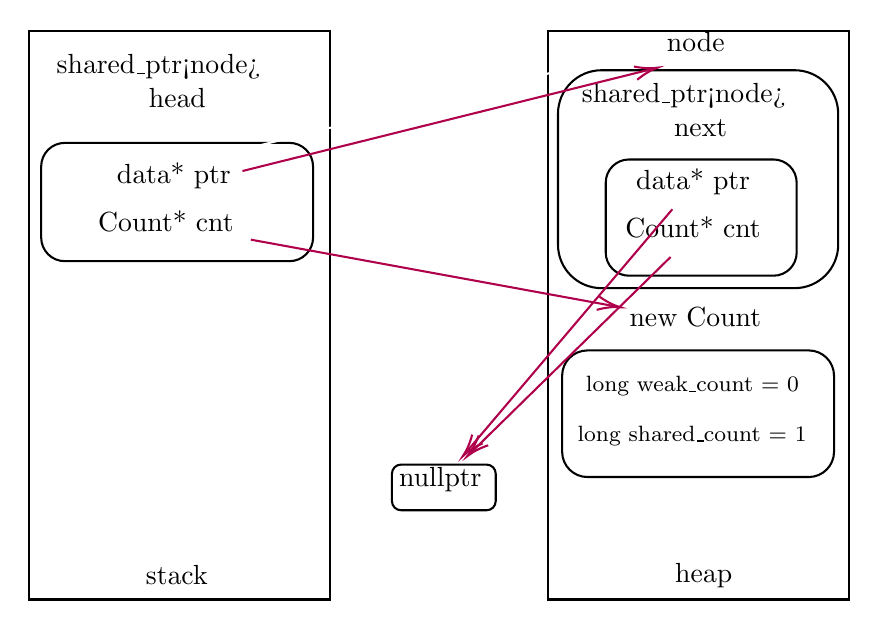
\begin{tikzpicture}[x=0.75pt,y=0.75pt,yscale=-1,xscale=1]
	%uncomment if require: \path (0,300); %set diagram left start at 0, and has height of 300
	
	%Rounded Rect [id:dp2187423114764504] 
	\draw   (139,77.4) .. controls (139,71.1) and (144.1,66) .. (150.4,66) -- (258.6,66) .. controls (264.9,66) and (270,71.1) .. (270,77.4) -- (270,111.6) .. controls (270,117.9) and (264.9,123) .. (258.6,123) -- (150.4,123) .. controls (144.1,123) and (139,117.9) .. (139,111.6) -- cycle ;
	%Shape: Rectangle [id:dp2941975065261839] 
	\draw   (133,12) -- (278,12) -- (278,286) -- (133,286) -- cycle ;
	%Shape: Rectangle [id:dp09704288189667065] 
	\draw   (383,12) -- (528,12) -- (528,286) -- (383,286) -- cycle ;
	%Rounded Rect [id:dp5478085044935208] 
	\draw   (388,52) .. controls (388,40.4) and (397.4,31) .. (409,31) -- (502,31) .. controls (513.6,31) and (523,40.4) .. (523,52) -- (523,115) .. controls (523,126.6) and (513.6,136) .. (502,136) -- (409,136) .. controls (397.4,136) and (388,126.6) .. (388,115) -- cycle ;
	%Rounded Rect [id:dp12609398185570142] 
	\draw   (411,85.2) .. controls (411,79.01) and (416.01,74) .. (422.2,74) -- (491.8,74) .. controls (497.99,74) and (503,79.01) .. (503,85.2) -- (503,118.8) .. controls (503,124.99) and (497.99,130) .. (491.8,130) -- (422.2,130) .. controls (416.01,130) and (411,124.99) .. (411,118.8) -- cycle ;
	%Rounded Rect [id:dp20297270277383261] 
	\draw   (390,178.2) .. controls (390,171.46) and (395.46,166) .. (402.2,166) -- (508.8,166) .. controls (515.54,166) and (521,171.46) .. (521,178.2) -- (521,214.8) .. controls (521,221.54) and (515.54,227) .. (508.8,227) -- (402.2,227) .. controls (395.46,227) and (390,221.54) .. (390,214.8) -- cycle ;
	%Rounded Rect [id:dp060261680865621337] 
	\draw   (308,225.4) .. controls (308,222.97) and (309.97,221) .. (312.4,221) -- (353.6,221) .. controls (356.03,221) and (358,222.97) .. (358,225.4) -- (358,238.6) .. controls (358,241.03) and (356.03,243) .. (353.6,243) -- (312.4,243) .. controls (309.97,243) and (308,241.03) .. (308,238.6) -- cycle ;
	
	% Text Node
	\draw (145,22) node [anchor=north west][inner sep=0.75pt]   [align=left] {shared\_ptr<node>\\ \ \ \ \ \ \ \ \ \ \ head};
	% Text Node
	\draw (439,11) node [anchor=north west][inner sep=0.75pt]   [align=left] {node};
	% Text Node
	\draw (174,74) node [anchor=north west][inner sep=0.75pt]   [align=left] {data* ptr};
	% Text Node
	\draw (165,97) node [anchor=north west][inner sep=0.75pt]   [align=left] {Count* cnt};
	% Text Node
	\draw (188,268) node [anchor=north west][inner sep=0.75pt]   [align=left] {stack};
	% Text Node
	\draw (443,267) node [anchor=north west][inner sep=0.75pt]   [align=left] {heap};
	% Text Node
	\draw (398,36) node [anchor=north west][inner sep=0.75pt]   [align=left] {shared\_ptr<node>\\ \ \ \ \ \ \ \ \ \ \ next};
	% Text Node
	\draw (424.2,77) node [anchor=north west][inner sep=0.75pt]   [align=left] {data* ptr};
	% Text Node
	\draw (419,100) node [anchor=north west][inner sep=0.75pt]   [align=left] {Count* cnt};
	% Text Node
	\draw (421,144) node [anchor=north west][inner sep=0.75pt]   [align=left] {new Count};
	% Text Node
	\draw (400,177) node [anchor=north west][inner sep=0.75pt]  [font=\footnotesize] [align=left] {long weak\_count = 0};
	% Text Node
	\draw (396,201) node [anchor=north west][inner sep=0.75pt]  [font=\footnotesize] [align=left] {long shared\_count = 1};
	% Text Node
	\draw (310,221) node [anchor=north west][inner sep=0.75pt]   [align=left] {nullptr};
	% Connection
	\draw [color={rgb, 255:red, 255; green, 255; blue, 255 }  ,draw opacity=1 ]   (233.01,70) -- (434.06,19.94) ;
	\draw [shift={(436,19.45)}, rotate = 166.02] [color={rgb, 255:red, 255; green, 255; blue, 255 }  ,draw opacity=1 ][line width=0.75]    (10.93,-3.29) .. controls (6.95,-1.4) and (3.31,-0.3) .. (0,0) .. controls (3.31,0.3) and (6.95,1.4) .. (10.93,3.29)   ;
	% Connection
	\draw [color={rgb, 255:red, 175; green, 0; blue, 75 }  ,draw opacity=1 ]   (236,79.56) -- (434.06,30.24) ;
	\draw [shift={(436,29.76)}, rotate = 166.02] [color={rgb, 255:red, 175; green, 0; blue, 75 }  ,draw opacity=1 ][line width=0.75]    (10.93,-3.29) .. controls (6.95,-1.4) and (3.31,-0.3) .. (0,0) .. controls (3.31,0.3) and (6.95,1.4) .. (10.93,3.29)   ;
	% Connection
	\draw [color={rgb, 255:red, 175; green, 0; blue, 75 }  ,draw opacity=1 ]   (240,112.63) -- (416.03,144.83) ;
	\draw [shift={(418,145.18)}, rotate = 190.36] [color={rgb, 255:red, 175; green, 0; blue, 75 }  ,draw opacity=1 ][line width=0.75]    (10.93,-3.29) .. controls (6.95,-1.4) and (3.31,-0.3) .. (0,0) .. controls (3.31,0.3) and (6.95,1.4) .. (10.93,3.29)   ;
	% Connection
	\draw [color={rgb, 255:red, 175; green, 0; blue, 75 }  ,draw opacity=1 ]   (443.09,98) -- (343.4,215.48) ;
	\draw [shift={(342.11,217)}, rotate = 310.32] [color={rgb, 255:red, 175; green, 0; blue, 75 }  ,draw opacity=1 ][line width=0.75]    (10.93,-3.29) .. controls (6.95,-1.4) and (3.31,-0.3) .. (0,0) .. controls (3.31,0.3) and (6.95,1.4) .. (10.93,3.29)   ;
	% Connection
	\draw [color={rgb, 255:red, 175; green, 0; blue, 75 }  ,draw opacity=1 ]   (442.24,121) -- (345.69,215.6) ;
	\draw [shift={(344.26,217)}, rotate = 315.59] [color={rgb, 255:red, 175; green, 0; blue, 75 }  ,draw opacity=1 ][line width=0.75]    (10.93,-3.29) .. controls (6.95,-1.4) and (3.31,-0.3) .. (0,0) .. controls (3.31,0.3) and (6.95,1.4) .. (10.93,3.29)   ;
	
	\end{tikzpicture}
	
{\tt (1)}
\end{center}
		\begin{center}



	\tikzset{every picture/.style={line width=0.75pt}} %set default line width to 0.75pt        

	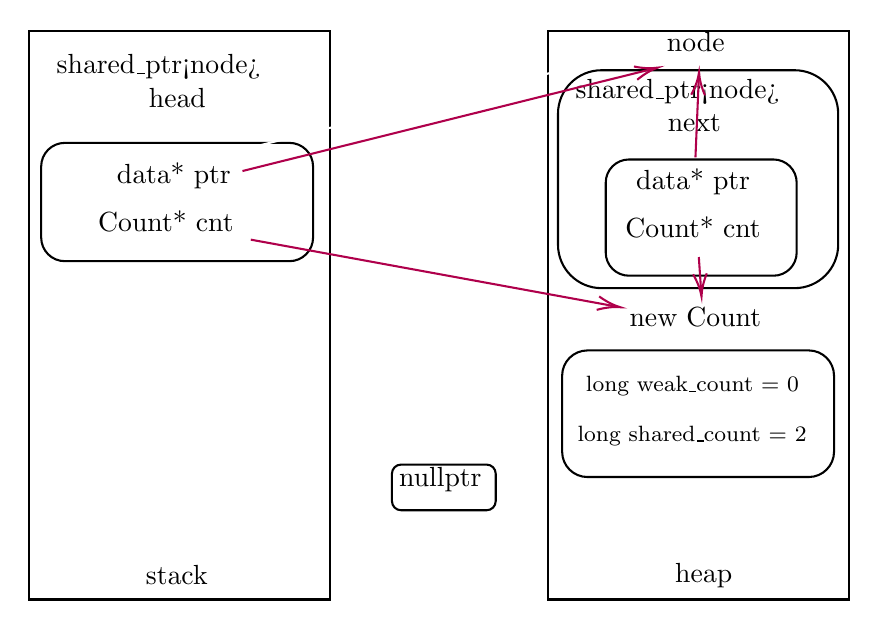
\begin{tikzpicture}[x=0.75pt,y=0.75pt,yscale=-1,xscale=1]
	%uncomment if require: \path (0,300); %set diagram left start at 0, and has height of 300
	
	%Rounded Rect [id:dp2187423114764504] 
	\draw   (139,77.4) .. controls (139,71.1) and (144.1,66) .. (150.4,66) -- (258.6,66) .. controls (264.9,66) and (270,71.1) .. (270,77.4) -- (270,111.6) .. controls (270,117.9) and (264.9,123) .. (258.6,123) -- (150.4,123) .. controls (144.1,123) and (139,117.9) .. (139,111.6) -- cycle ;
	%Shape: Rectangle [id:dp2941975065261839] 
	\draw   (133,12) -- (278,12) -- (278,286) -- (133,286) -- cycle ;
	%Shape: Rectangle [id:dp09704288189667065] 
	\draw   (383,12) -- (528,12) -- (528,286) -- (383,286) -- cycle ;
	%Rounded Rect [id:dp5478085044935208] 
	\draw   (388,52) .. controls (388,40.4) and (397.4,31) .. (409,31) -- (502,31) .. controls (513.6,31) and (523,40.4) .. (523,52) -- (523,115) .. controls (523,126.6) and (513.6,136) .. (502,136) -- (409,136) .. controls (397.4,136) and (388,126.6) .. (388,115) -- cycle ;
	%Rounded Rect [id:dp12609398185570142] 
	\draw   (411,85.2) .. controls (411,79.01) and (416.01,74) .. (422.2,74) -- (491.8,74) .. controls (497.99,74) and (503,79.01) .. (503,85.2) -- (503,118.8) .. controls (503,124.99) and (497.99,130) .. (491.8,130) -- (422.2,130) .. controls (416.01,130) and (411,124.99) .. (411,118.8) -- cycle ;
	%Rounded Rect [id:dp20297270277383261] 
	\draw   (390,178.2) .. controls (390,171.46) and (395.46,166) .. (402.2,166) -- (508.8,166) .. controls (515.54,166) and (521,171.46) .. (521,178.2) -- (521,214.8) .. controls (521,221.54) and (515.54,227) .. (508.8,227) -- (402.2,227) .. controls (395.46,227) and (390,221.54) .. (390,214.8) -- cycle ;
	%Rounded Rect [id:dp060261680865621337] 
	\draw   (308,225.4) .. controls (308,222.97) and (309.97,221) .. (312.4,221) -- (353.6,221) .. controls (356.03,221) and (358,222.97) .. (358,225.4) -- (358,238.6) .. controls (358,241.03) and (356.03,243) .. (353.6,243) -- (312.4,243) .. controls (309.97,243) and (308,241.03) .. (308,238.6) -- cycle ;
	
	% Text Node
	\draw (145,22) node [anchor=north west][inner sep=0.75pt]   [align=left] {shared\_ptr<node>\\ \ \ \ \ \ \ \ \ \ \ head};
	% Text Node
	\draw (439,11) node [anchor=north west][inner sep=0.75pt]   [align=left] {node};
	% Text Node
	\draw (174,74) node [anchor=north west][inner sep=0.75pt]   [align=left] {data* ptr};
	% Text Node
	\draw (165,97) node [anchor=north west][inner sep=0.75pt]   [align=left] {Count* cnt};
	% Text Node
	\draw (188,268) node [anchor=north west][inner sep=0.75pt]   [align=left] {stack};
	% Text Node
	\draw (443,267) node [anchor=north west][inner sep=0.75pt]   [align=left] {heap};
	% Text Node
	\draw (395,34) node [anchor=north west][inner sep=0.75pt]   [align=left] {shared\_ptr<node>\\ \ \ \ \ \ \ \ \ \ \ next};
	% Text Node
	\draw (424.2,77) node [anchor=north west][inner sep=0.75pt]   [align=left] {data* ptr};
	% Text Node
	\draw (419,100) node [anchor=north west][inner sep=0.75pt]   [align=left] {Count* cnt};
	% Text Node
	\draw (421,144) node [anchor=north west][inner sep=0.75pt]   [align=left] {new Count};
	% Text Node
	\draw (400,177) node [anchor=north west][inner sep=0.75pt]  [font=\footnotesize] [align=left] {long weak\_count = 0};
	% Text Node
	\draw (396,201) node [anchor=north west][inner sep=0.75pt]  [font=\footnotesize] [align=left] {long shared\_count = 2};
	% Text Node
	\draw (310,221) node [anchor=north west][inner sep=0.75pt]   [align=left] {nullptr};
	% Connection
	\draw [color={rgb, 255:red, 255; green, 255; blue, 255 }  ,draw opacity=1 ]   (233.01,70) -- (434.06,19.94) ;
	\draw [shift={(436,19.45)}, rotate = 166.02] [color={rgb, 255:red, 255; green, 255; blue, 255 }  ,draw opacity=1 ][line width=0.75]    (10.93,-3.29) .. controls (6.95,-1.4) and (3.31,-0.3) .. (0,0) .. controls (3.31,0.3) and (6.95,1.4) .. (10.93,3.29)   ;
	% Connection
	\draw [color={rgb, 255:red, 175; green, 0; blue, 75 }  ,draw opacity=1 ]   (236,79.56) -- (434.06,30.24) ;
	\draw [shift={(436,29.76)}, rotate = 166.02] [color={rgb, 255:red, 175; green, 0; blue, 75 }  ,draw opacity=1 ][line width=0.75]    (10.93,-3.29) .. controls (6.95,-1.4) and (3.31,-0.3) .. (0,0) .. controls (3.31,0.3) and (6.95,1.4) .. (10.93,3.29)   ;
	% Connection
	\draw [color={rgb, 255:red, 175; green, 0; blue, 75 }  ,draw opacity=1 ]   (240,112.63) -- (416.03,144.83) ;
	\draw [shift={(418,145.18)}, rotate = 190.36] [color={rgb, 255:red, 175; green, 0; blue, 75 }  ,draw opacity=1 ][line width=0.75]    (10.93,-3.29) .. controls (6.95,-1.4) and (3.31,-0.3) .. (0,0) .. controls (3.31,0.3) and (6.95,1.4) .. (10.93,3.29)   ;
	% Connection
	\draw [color={rgb, 255:red, 175; green, 0; blue, 75 }  ,draw opacity=1 ]   (454.23,73) -- (455.88,34) ;
	\draw [shift={(455.97,32)}, rotate = 92.43] [color={rgb, 255:red, 175; green, 0; blue, 75 }  ,draw opacity=1 ][line width=0.75]    (10.93,-3.29) .. controls (6.95,-1.4) and (3.31,-0.3) .. (0,0) .. controls (3.31,0.3) and (6.95,1.4) .. (10.93,3.29)   ;
	% Connection
	\draw [color={rgb, 255:red, 175; green, 0; blue, 75 }  ,draw opacity=1 ]   (455.85,121) -- (457.01,138) ;
	\draw [shift={(457.15,140)}, rotate = 266.1] [color={rgb, 255:red, 175; green, 0; blue, 75 }  ,draw opacity=1 ][line width=0.75]    (10.93,-3.29) .. controls (6.95,-1.4) and (3.31,-0.3) .. (0,0) .. controls (3.31,0.3) and (6.95,1.4) .. (10.93,3.29)   ;
	
	\end{tikzpicture}

{\tt (2)}
\end{center}
		\begin{center}

\tikzset{every picture/.style={line width=0.75pt}} %set default line width to 0.75pt        

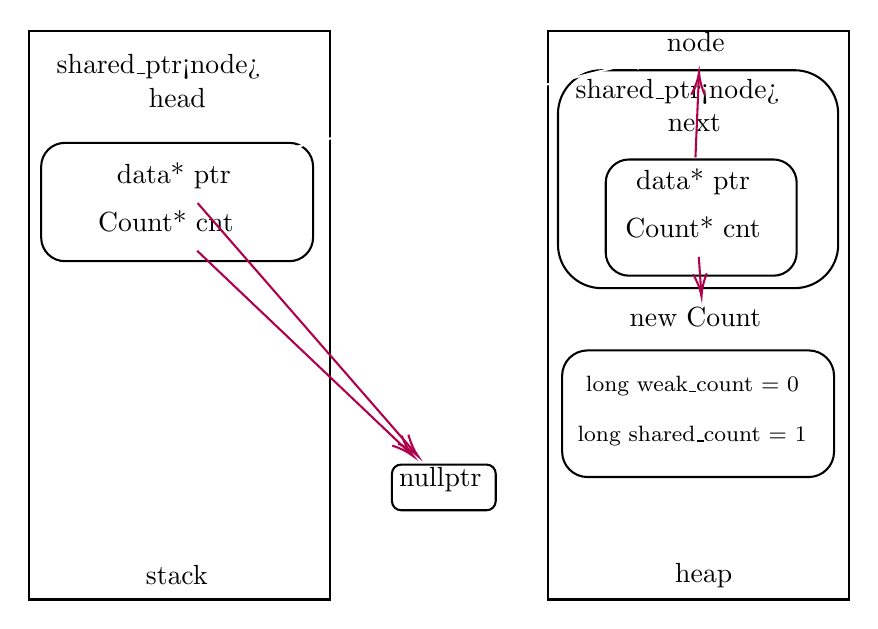
\begin{tikzpicture}[x=0.75pt,y=0.75pt,yscale=-1,xscale=1]
%uncomment if require: \path (0,300); %set diagram left start at 0, and has height of 300

%Rounded Rect [id:dp2187423114764504] 
\draw   (139,77.4) .. controls (139,71.1) and (144.1,66) .. (150.4,66) -- (258.6,66) .. controls (264.9,66) and (270,71.1) .. (270,77.4) -- (270,111.6) .. controls (270,117.9) and (264.9,123) .. (258.6,123) -- (150.4,123) .. controls (144.1,123) and (139,117.9) .. (139,111.6) -- cycle ;
%Shape: Rectangle [id:dp2941975065261839] 
\draw   (133,12) -- (278,12) -- (278,286) -- (133,286) -- cycle ;
%Shape: Rectangle [id:dp09704288189667065] 
\draw   (383,12) -- (528,12) -- (528,286) -- (383,286) -- cycle ;
%Rounded Rect [id:dp5478085044935208] 
\draw   (388,52) .. controls (388,40.4) and (397.4,31) .. (409,31) -- (502,31) .. controls (513.6,31) and (523,40.4) .. (523,52) -- (523,115) .. controls (523,126.6) and (513.6,136) .. (502,136) -- (409,136) .. controls (397.4,136) and (388,126.6) .. (388,115) -- cycle ;
%Rounded Rect [id:dp12609398185570142] 
\draw   (411,85.2) .. controls (411,79.01) and (416.01,74) .. (422.2,74) -- (491.8,74) .. controls (497.99,74) and (503,79.01) .. (503,85.2) -- (503,118.8) .. controls (503,124.99) and (497.99,130) .. (491.8,130) -- (422.2,130) .. controls (416.01,130) and (411,124.99) .. (411,118.8) -- cycle ;
%Rounded Rect [id:dp20297270277383261] 
\draw   (390,178.2) .. controls (390,171.46) and (395.46,166) .. (402.2,166) -- (508.8,166) .. controls (515.54,166) and (521,171.46) .. (521,178.2) -- (521,214.8) .. controls (521,221.54) and (515.54,227) .. (508.8,227) -- (402.2,227) .. controls (395.46,227) and (390,221.54) .. (390,214.8) -- cycle ;
%Rounded Rect [id:dp060261680865621337] 
\draw   (308,225.4) .. controls (308,222.97) and (309.97,221) .. (312.4,221) -- (353.6,221) .. controls (356.03,221) and (358,222.97) .. (358,225.4) -- (358,238.6) .. controls (358,241.03) and (356.03,243) .. (353.6,243) -- (312.4,243) .. controls (309.97,243) and (308,241.03) .. (308,238.6) -- cycle ;

% Text Node
\draw (145,22) node [anchor=north west][inner sep=0.75pt]   [align=left] {shared\_ptr<node>\\ \ \ \ \ \ \ \ \ \ \ head};
% Text Node
\draw (439,11) node [anchor=north west][inner sep=0.75pt]   [align=left] {node};
% Text Node
\draw (174,74) node [anchor=north west][inner sep=0.75pt]   [align=left] {data* ptr};
% Text Node
\draw (165,97) node [anchor=north west][inner sep=0.75pt]   [align=left] {Count* cnt};
% Text Node
\draw (188,268) node [anchor=north west][inner sep=0.75pt]   [align=left] {stack};
% Text Node
\draw (443,267) node [anchor=north west][inner sep=0.75pt]   [align=left] {heap};
% Text Node
\draw (395,34) node [anchor=north west][inner sep=0.75pt]   [align=left] {shared\_ptr<node>\\ \ \ \ \ \ \ \ \ \ \ next};
% Text Node
\draw (424.2,77) node [anchor=north west][inner sep=0.75pt]   [align=left] {data* ptr};
% Text Node
\draw (419,100) node [anchor=north west][inner sep=0.75pt]   [align=left] {Count* cnt};
% Text Node
\draw (421,144) node [anchor=north west][inner sep=0.75pt]   [align=left] {new Count};
% Text Node
\draw (400,177) node [anchor=north west][inner sep=0.75pt]  [font=\footnotesize] [align=left] {long weak\_count = 0};
% Text Node
\draw (396,201) node [anchor=north west][inner sep=0.75pt]  [font=\footnotesize] [align=left] {long shared\_count = 1};
% Text Node
\draw (310,221) node [anchor=north west][inner sep=0.75pt]   [align=left] {nullptr};
% Connection
\draw [color={rgb, 255:red, 255; green, 255; blue, 255 }  ,draw opacity=1 ]   (236,74.41) -- (434.06,25.09) ;
\draw [shift={(436,24.6)}, rotate = 166.02] [color={rgb, 255:red, 255; green, 255; blue, 255 }  ,draw opacity=1 ][line width=0.75]    (10.93,-3.29) .. controls (6.95,-1.4) and (3.31,-0.3) .. (0,0) .. controls (3.31,0.3) and (6.95,1.4) .. (10.93,3.29)   ;
% Connection
\draw [color={rgb, 255:red, 175; green, 0; blue, 75 }  ,draw opacity=1 ]   (454.23,73) -- (455.88,34) ;
\draw [shift={(455.97,32)}, rotate = 92.43] [color={rgb, 255:red, 175; green, 0; blue, 75 }  ,draw opacity=1 ][line width=0.75]    (10.93,-3.29) .. controls (6.95,-1.4) and (3.31,-0.3) .. (0,0) .. controls (3.31,0.3) and (6.95,1.4) .. (10.93,3.29)   ;
% Connection
\draw [color={rgb, 255:red, 175; green, 0; blue, 75 }  ,draw opacity=1 ]   (455.85,121) -- (457.01,138) ;
\draw [shift={(457.15,140)}, rotate = 266.1] [color={rgb, 255:red, 175; green, 0; blue, 75 }  ,draw opacity=1 ][line width=0.75]    (10.93,-3.29) .. controls (6.95,-1.4) and (3.31,-0.3) .. (0,0) .. controls (3.31,0.3) and (6.95,1.4) .. (10.93,3.29)   ;
% Connection
\draw [color={rgb, 255:red, 175; green, 0; blue, 75 }  ,draw opacity=1 ]   (214.38,95) -- (319.3,215.49) ;
\draw [shift={(320.62,217)}, rotate = 228.95] [color={rgb, 255:red, 175; green, 0; blue, 75 }  ,draw opacity=1 ][line width=0.75]    (10.93,-3.29) .. controls (6.95,-1.4) and (3.31,-0.3) .. (0,0) .. controls (3.31,0.3) and (6.95,1.4) .. (10.93,3.29)   ;
% Connection
\draw [color={rgb, 255:red, 175; green, 0; blue, 75 }  ,draw opacity=1 ]   (214.16,118) -- (316.89,215.62) ;
\draw [shift={(318.34,217)}, rotate = 223.54] [color={rgb, 255:red, 175; green, 0; blue, 75 }  ,draw opacity=1 ][line width=0.75]    (10.93,-3.29) .. controls (6.95,-1.4) and (3.31,-0.3) .. (0,0) .. controls (3.31,0.3) and (6.95,1.4) .. (10.93,3.29)   ;

\end{tikzpicture}

{\tt (3)}

\end{center}
		\item 可以看出引用计数一直在正常工作, 问题在于当栈上{\tt head}主动调用{\tt reset}进行析构, 
				或者被动析构时, 此时引用计数为2, 因此不会释放{\tt node}, 也就不会释放{\tt next},
				而位于堆上的{\tt next}不会自动析构, 就造成了内存泄露
		\item 当一个含有{\tt shared\_ptr}的对象被构造在堆上, 那么{\tt shared\_ptr}本身也就在堆上, 
				若它指向另一个堆对象, 则该堆对象析构同步于{\tt shared\_ptr}本身析构, 而{\tt shared\_ptr}
				本身析构同步于自身所处的对象析构, 则若这两个对象是同一对象, 或者更广泛的连成一个环, 它们的析构是
				同步的, 那么就只能主动调用其中一个{\tt shared\_ptr}进行析构才能释放, 此时这个{\tt shared\_ptr}与
				普通指针并无区别, 一样需要主动{\tt delete}, 失去了它作为智能指针的意义
		\item 此时我们引入{\tt weak\_ptr}, {\tt weak\_ptr}只能指向{\tt shared\_ptr}指向的对象, 而它自身不实际拥有任何对象
		\begin{center}

\tikzset{every picture/.style={line width=0.75pt}} %set default line width to 0.75pt        

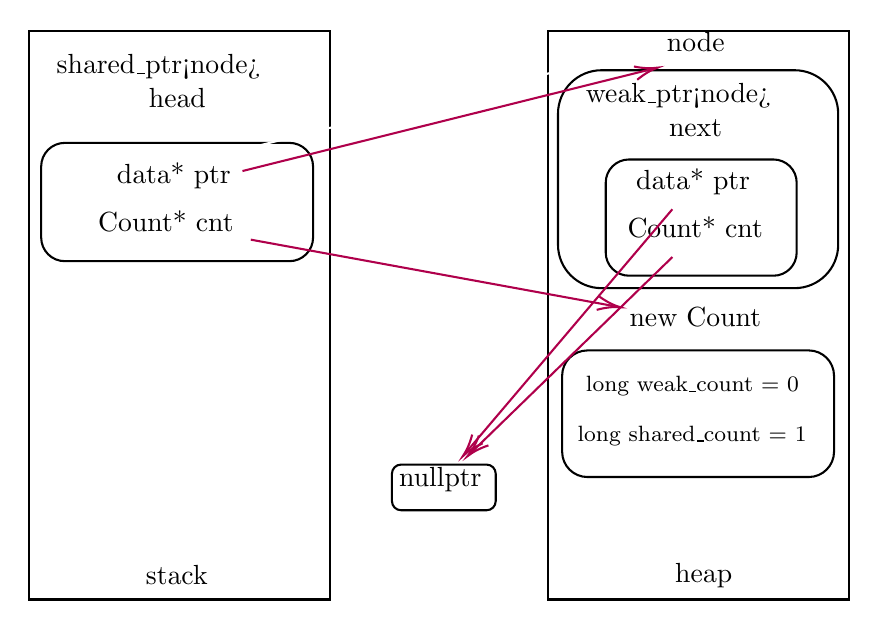
\begin{tikzpicture}[x=0.75pt,y=0.75pt,yscale=-1,xscale=1]
%uncomment if require: \path (0,300); %set diagram left start at 0, and has height of 300

%Rounded Rect [id:dp2187423114764504] 
\draw   (139,77.4) .. controls (139,71.1) and (144.1,66) .. (150.4,66) -- (258.6,66) .. controls (264.9,66) and (270,71.1) .. (270,77.4) -- (270,111.6) .. controls (270,117.9) and (264.9,123) .. (258.6,123) -- (150.4,123) .. controls (144.1,123) and (139,117.9) .. (139,111.6) -- cycle ;
%Shape: Rectangle [id:dp2941975065261839] 
\draw   (133,12) -- (278,12) -- (278,286) -- (133,286) -- cycle ;
%Shape: Rectangle [id:dp09704288189667065] 
\draw   (383,12) -- (528,12) -- (528,286) -- (383,286) -- cycle ;
%Rounded Rect [id:dp5478085044935208] 
\draw   (388,52) .. controls (388,40.4) and (397.4,31) .. (409,31) -- (502,31) .. controls (513.6,31) and (523,40.4) .. (523,52) -- (523,115) .. controls (523,126.6) and (513.6,136) .. (502,136) -- (409,136) .. controls (397.4,136) and (388,126.6) .. (388,115) -- cycle ;
%Rounded Rect [id:dp12609398185570142] 
\draw   (411,85.2) .. controls (411,79.01) and (416.01,74) .. (422.2,74) -- (491.8,74) .. controls (497.99,74) and (503,79.01) .. (503,85.2) -- (503,118.8) .. controls (503,124.99) and (497.99,130) .. (491.8,130) -- (422.2,130) .. controls (416.01,130) and (411,124.99) .. (411,118.8) -- cycle ;
%Rounded Rect [id:dp20297270277383261] 
\draw   (390,178.2) .. controls (390,171.46) and (395.46,166) .. (402.2,166) -- (508.8,166) .. controls (515.54,166) and (521,171.46) .. (521,178.2) -- (521,214.8) .. controls (521,221.54) and (515.54,227) .. (508.8,227) -- (402.2,227) .. controls (395.46,227) and (390,221.54) .. (390,214.8) -- cycle ;
%Rounded Rect [id:dp060261680865621337] 
\draw   (308,225.4) .. controls (308,222.97) and (309.97,221) .. (312.4,221) -- (353.6,221) .. controls (356.03,221) and (358,222.97) .. (358,225.4) -- (358,238.6) .. controls (358,241.03) and (356.03,243) .. (353.6,243) -- (312.4,243) .. controls (309.97,243) and (308,241.03) .. (308,238.6) -- cycle ;

% Text Node
\draw (145,22) node [anchor=north west][inner sep=0.75pt]   [align=left] {shared\_ptr<node>\\ \ \ \ \ \ \ \ \ \ \ head};
% Text Node
\draw (439,11) node [anchor=north west][inner sep=0.75pt]   [align=left] {node};
% Text Node
\draw (174,74) node [anchor=north west][inner sep=0.75pt]   [align=left] {data* ptr};
% Text Node
\draw (165,97) node [anchor=north west][inner sep=0.75pt]   [align=left] {Count* cnt};
% Text Node
\draw (188,268) node [anchor=north west][inner sep=0.75pt]   [align=left] {stack};
% Text Node
\draw (443,267) node [anchor=north west][inner sep=0.75pt]   [align=left] {heap};
% Text Node
\draw (400,36) node [anchor=north west][inner sep=0.75pt]   [align=left] {weak\_ptr<node>\\ \ \ \ \ \ \ \ \ \ next};
% Text Node
\draw (424.2,77) node [anchor=north west][inner sep=0.75pt]   [align=left] {data* ptr};
% Text Node
\draw (420,100) node [anchor=north west][inner sep=0.75pt]   [align=left] {Count* cnt};
% Text Node
\draw (421,144) node [anchor=north west][inner sep=0.75pt]   [align=left] {new Count};
% Text Node
\draw (400,177) node [anchor=north west][inner sep=0.75pt]  [font=\footnotesize] [align=left] {long weak\_count = 0};
% Text Node
\draw (396,201) node [anchor=north west][inner sep=0.75pt]  [font=\footnotesize] [align=left] {long shared\_count = 1};
% Text Node
\draw (310,221) node [anchor=north west][inner sep=0.75pt]   [align=left] {nullptr};
% Connection
\draw [color={rgb, 255:red, 255; green, 255; blue, 255 }  ,draw opacity=1 ]   (233.01,70) -- (434.06,19.94) ;
\draw [shift={(436,19.45)}, rotate = 166.02] [color={rgb, 255:red, 255; green, 255; blue, 255 }  ,draw opacity=1 ][line width=0.75]    (10.93,-3.29) .. controls (6.95,-1.4) and (3.31,-0.3) .. (0,0) .. controls (3.31,0.3) and (6.95,1.4) .. (10.93,3.29)   ;
% Connection
\draw [color={rgb, 255:red, 175; green, 0; blue, 75 }  ,draw opacity=1 ]   (236,79.56) -- (434.06,30.24) ;
\draw [shift={(436,29.76)}, rotate = 166.02] [color={rgb, 255:red, 175; green, 0; blue, 75 }  ,draw opacity=1 ][line width=0.75]    (10.93,-3.29) .. controls (6.95,-1.4) and (3.31,-0.3) .. (0,0) .. controls (3.31,0.3) and (6.95,1.4) .. (10.93,3.29)   ;
% Connection
\draw [color={rgb, 255:red, 175; green, 0; blue, 75 }  ,draw opacity=1 ]   (240,112.63) -- (416.03,144.83) ;
\draw [shift={(418,145.18)}, rotate = 190.36] [color={rgb, 255:red, 175; green, 0; blue, 75 }  ,draw opacity=1 ][line width=0.75]    (10.93,-3.29) .. controls (6.95,-1.4) and (3.31,-0.3) .. (0,0) .. controls (3.31,0.3) and (6.95,1.4) .. (10.93,3.29)   ;
% Connection
\draw [color={rgb, 255:red, 175; green, 0; blue, 75 }  ,draw opacity=1 ]   (443.09,98) -- (343.4,215.48) ;
\draw [shift={(342.11,217)}, rotate = 310.32] [color={rgb, 255:red, 175; green, 0; blue, 75 }  ,draw opacity=1 ][line width=0.75]    (10.93,-3.29) .. controls (6.95,-1.4) and (3.31,-0.3) .. (0,0) .. controls (3.31,0.3) and (6.95,1.4) .. (10.93,3.29)   ;
% Connection
\draw [color={rgb, 255:red, 175; green, 0; blue, 75 }  ,draw opacity=1 ]   (443.14,121) -- (345.8,215.61) ;
\draw [shift={(344.36,217)}, rotate = 315.82] [color={rgb, 255:red, 175; green, 0; blue, 75 }  ,draw opacity=1 ][line width=0.75]    (10.93,-3.29) .. controls (6.95,-1.4) and (3.31,-0.3) .. (0,0) .. controls (3.31,0.3) and (6.95,1.4) .. (10.93,3.29)   ;

\end{tikzpicture}

{\tt (1)}	
\end{center}

		\begin{center}



\tikzset{every picture/.style={line width=0.75pt}} %set default line width to 0.75pt        

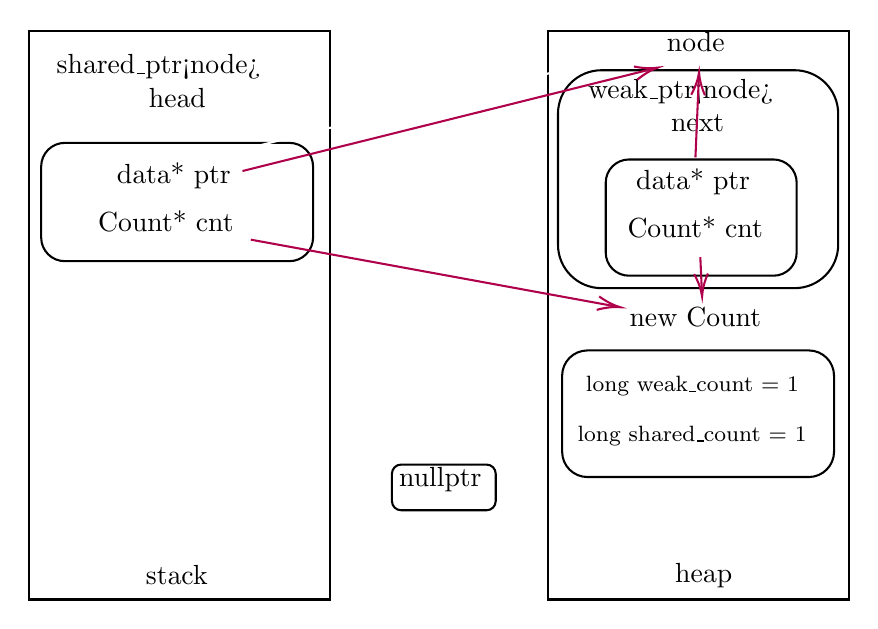
\begin{tikzpicture}[x=0.75pt,y=0.75pt,yscale=-1,xscale=1]
%uncomment if require: \path (0,300); %set diagram left start at 0, and has height of 300

%Rounded Rect [id:dp2187423114764504] 
\draw   (139,77.4) .. controls (139,71.1) and (144.1,66) .. (150.4,66) -- (258.6,66) .. controls (264.9,66) and (270,71.1) .. (270,77.4) -- (270,111.6) .. controls (270,117.9) and (264.9,123) .. (258.6,123) -- (150.4,123) .. controls (144.1,123) and (139,117.9) .. (139,111.6) -- cycle ;
%Shape: Rectangle [id:dp2941975065261839] 
\draw   (133,12) -- (278,12) -- (278,286) -- (133,286) -- cycle ;
%Shape: Rectangle [id:dp09704288189667065] 
\draw   (383,12) -- (528,12) -- (528,286) -- (383,286) -- cycle ;
%Rounded Rect [id:dp5478085044935208] 
\draw   (388,52) .. controls (388,40.4) and (397.4,31) .. (409,31) -- (502,31) .. controls (513.6,31) and (523,40.4) .. (523,52) -- (523,115) .. controls (523,126.6) and (513.6,136) .. (502,136) -- (409,136) .. controls (397.4,136) and (388,126.6) .. (388,115) -- cycle ;
%Rounded Rect [id:dp12609398185570142] 
\draw   (411,85.2) .. controls (411,79.01) and (416.01,74) .. (422.2,74) -- (491.8,74) .. controls (497.99,74) and (503,79.01) .. (503,85.2) -- (503,118.8) .. controls (503,124.99) and (497.99,130) .. (491.8,130) -- (422.2,130) .. controls (416.01,130) and (411,124.99) .. (411,118.8) -- cycle ;
%Rounded Rect [id:dp20297270277383261] 
\draw   (390,178.2) .. controls (390,171.46) and (395.46,166) .. (402.2,166) -- (508.8,166) .. controls (515.54,166) and (521,171.46) .. (521,178.2) -- (521,214.8) .. controls (521,221.54) and (515.54,227) .. (508.8,227) -- (402.2,227) .. controls (395.46,227) and (390,221.54) .. (390,214.8) -- cycle ;
%Rounded Rect [id:dp060261680865621337] 
\draw   (308,225.4) .. controls (308,222.97) and (309.97,221) .. (312.4,221) -- (353.6,221) .. controls (356.03,221) and (358,222.97) .. (358,225.4) -- (358,238.6) .. controls (358,241.03) and (356.03,243) .. (353.6,243) -- (312.4,243) .. controls (309.97,243) and (308,241.03) .. (308,238.6) -- cycle ;

% Text Node
\draw (145,22) node [anchor=north west][inner sep=0.75pt]   [align=left] {shared\_ptr<node>\\ \ \ \ \ \ \ \ \ \ \ head};
% Text Node
\draw (439,11) node [anchor=north west][inner sep=0.75pt]   [align=left] {node};
% Text Node
\draw (174,74) node [anchor=north west][inner sep=0.75pt]   [align=left] {data* ptr};
% Text Node
\draw (165,97) node [anchor=north west][inner sep=0.75pt]   [align=left] {Count* cnt};
% Text Node
\draw (188,268) node [anchor=north west][inner sep=0.75pt]   [align=left] {stack};
% Text Node
\draw (443,267) node [anchor=north west][inner sep=0.75pt]   [align=left] {heap};
% Text Node
\draw (401,34) node [anchor=north west][inner sep=0.75pt]   [align=left] {weak\_ptr<node>\\ \ \ \ \ \ \ \ \ \ next};
% Text Node
\draw (424.2,77) node [anchor=north west][inner sep=0.75pt]   [align=left] {data* ptr};
% Text Node
\draw (420,100) node [anchor=north west][inner sep=0.75pt]   [align=left] {Count* cnt};
% Text Node
\draw (421,144) node [anchor=north west][inner sep=0.75pt]   [align=left] {new Count};
% Text Node
\draw (400,177) node [anchor=north west][inner sep=0.75pt]  [font=\footnotesize] [align=left] {long weak\_count = 1};
% Text Node
\draw (396,201) node [anchor=north west][inner sep=0.75pt]  [font=\footnotesize] [align=left] {long shared\_count = 1};
% Text Node
\draw (310,221) node [anchor=north west][inner sep=0.75pt]   [align=left] {nullptr};
% Connection
\draw [color={rgb, 255:red, 255; green, 255; blue, 255 }  ,draw opacity=1 ]   (233.01,70) -- (434.06,19.94) ;
\draw [shift={(436,19.45)}, rotate = 166.02] [color={rgb, 255:red, 255; green, 255; blue, 255 }  ,draw opacity=1 ][line width=0.75]    (10.93,-3.29) .. controls (6.95,-1.4) and (3.31,-0.3) .. (0,0) .. controls (3.31,0.3) and (6.95,1.4) .. (10.93,3.29)   ;
% Connection
\draw [color={rgb, 255:red, 175; green, 0; blue, 75 }  ,draw opacity=1 ]   (236,79.56) -- (434.06,30.24) ;
\draw [shift={(436,29.76)}, rotate = 166.02] [color={rgb, 255:red, 175; green, 0; blue, 75 }  ,draw opacity=1 ][line width=0.75]    (10.93,-3.29) .. controls (6.95,-1.4) and (3.31,-0.3) .. (0,0) .. controls (3.31,0.3) and (6.95,1.4) .. (10.93,3.29)   ;
% Connection
\draw [color={rgb, 255:red, 175; green, 0; blue, 75 }  ,draw opacity=1 ]   (240,112.63) -- (416.03,144.83) ;
\draw [shift={(418,145.18)}, rotate = 190.36] [color={rgb, 255:red, 175; green, 0; blue, 75 }  ,draw opacity=1 ][line width=0.75]    (10.93,-3.29) .. controls (6.95,-1.4) and (3.31,-0.3) .. (0,0) .. controls (3.31,0.3) and (6.95,1.4) .. (10.93,3.29)   ;
% Connection
\draw [color={rgb, 255:red, 175; green, 0; blue, 75 }  ,draw opacity=1 ]   (454.23,73) -- (455.88,34) ;
\draw [shift={(455.97,32)}, rotate = 92.43] [color={rgb, 255:red, 175; green, 0; blue, 75 }  ,draw opacity=1 ][line width=0.75]    (10.93,-3.29) .. controls (6.95,-1.4) and (3.31,-0.3) .. (0,0) .. controls (3.31,0.3) and (6.95,1.4) .. (10.93,3.29)   ;
% Connection
\draw [color={rgb, 255:red, 175; green, 0; blue, 75 }  ,draw opacity=1 ]   (456.57,121) -- (457.34,138) ;
\draw [shift={(457.43,140)}, rotate = 267.4] [color={rgb, 255:red, 175; green, 0; blue, 75 }  ,draw opacity=1 ][line width=0.75]    (10.93,-3.29) .. controls (6.95,-1.4) and (3.31,-0.3) .. (0,0) .. controls (3.31,0.3) and (6.95,1.4) .. (10.93,3.29)   ;

\end{tikzpicture}

{\tt (2)}	
\end{center}
		\begin{center}




	\tikzset{every picture/.style={line width=0.75pt}} %set default line width to 0.75pt        

	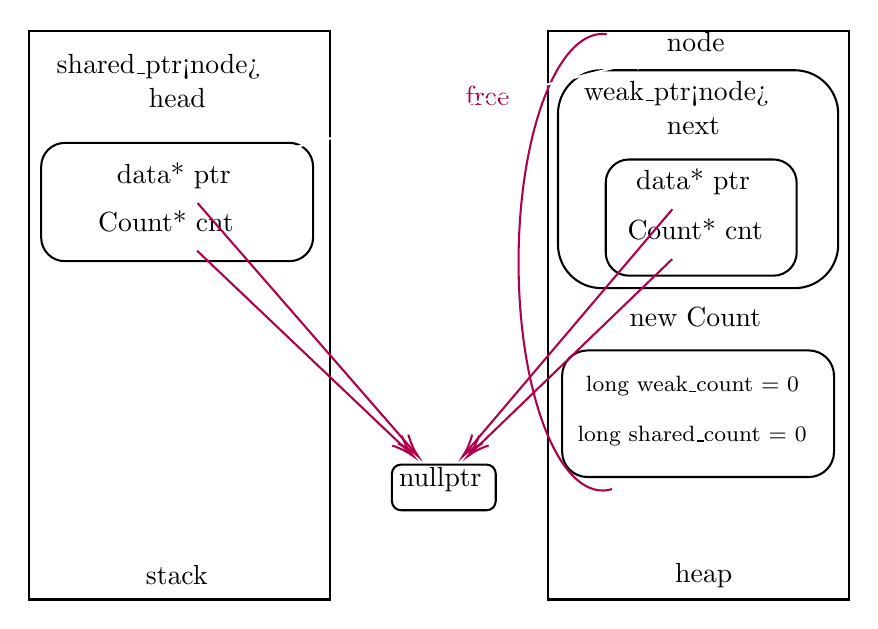
\begin{tikzpicture}[x=0.75pt,y=0.75pt,yscale=-1,xscale=1]
	%uncomment if require: \path (0,300); %set diagram left start at 0, and has height of 300
	
	%Rounded Rect [id:dp2187423114764504] 
	\draw   (139,77.4) .. controls (139,71.1) and (144.1,66) .. (150.4,66) -- (258.6,66) .. controls (264.9,66) and (270,71.1) .. (270,77.4) -- (270,111.6) .. controls (270,117.9) and (264.9,123) .. (258.6,123) -- (150.4,123) .. controls (144.1,123) and (139,117.9) .. (139,111.6) -- cycle ;
	%Shape: Rectangle [id:dp2941975065261839] 
	\draw   (133,12) -- (278,12) -- (278,286) -- (133,286) -- cycle ;
	%Shape: Rectangle [id:dp09704288189667065] 
	\draw   (383,12) -- (528,12) -- (528,286) -- (383,286) -- cycle ;
	%Rounded Rect [id:dp5478085044935208] 
	\draw   (388,52) .. controls (388,40.4) and (397.4,31) .. (409,31) -- (502,31) .. controls (513.6,31) and (523,40.4) .. (523,52) -- (523,115) .. controls (523,126.6) and (513.6,136) .. (502,136) -- (409,136) .. controls (397.4,136) and (388,126.6) .. (388,115) -- cycle ;
	%Rounded Rect [id:dp12609398185570142] 
	\draw   (411,85.2) .. controls (411,79.01) and (416.01,74) .. (422.2,74) -- (491.8,74) .. controls (497.99,74) and (503,79.01) .. (503,85.2) -- (503,118.8) .. controls (503,124.99) and (497.99,130) .. (491.8,130) -- (422.2,130) .. controls (416.01,130) and (411,124.99) .. (411,118.8) -- cycle ;
	%Rounded Rect [id:dp20297270277383261] 
	\draw   (390,178.2) .. controls (390,171.46) and (395.46,166) .. (402.2,166) -- (508.8,166) .. controls (515.54,166) and (521,171.46) .. (521,178.2) -- (521,214.8) .. controls (521,221.54) and (515.54,227) .. (508.8,227) -- (402.2,227) .. controls (395.46,227) and (390,221.54) .. (390,214.8) -- cycle ;
	%Rounded Rect [id:dp060261680865621337] 
	\draw   (308,225.4) .. controls (308,222.97) and (309.97,221) .. (312.4,221) -- (353.6,221) .. controls (356.03,221) and (358,222.97) .. (358,225.4) -- (358,238.6) .. controls (358,241.03) and (356.03,243) .. (353.6,243) -- (312.4,243) .. controls (309.97,243) and (308,241.03) .. (308,238.6) -- cycle ;
	%Shape: Arc [id:dp11695516109199944] 
	\draw  [draw opacity=0] (414.02,232.82) .. controls (412.54,233.27) and (411.03,233.5) .. (409.5,233.5) .. controls (387.13,233.5) and (369,184.25) .. (369,123.5) .. controls (369,62.75) and (387.13,13.5) .. (409.5,13.5) .. controls (410.17,13.5) and (410.83,13.54) .. (411.49,13.63) -- (409.5,123.5) -- cycle ; \draw  [color={rgb, 255:red, 175; green, 0; blue, 75 }  ,draw opacity=1 ] (414.02,232.82) .. controls (412.54,233.27) and (411.03,233.5) .. (409.5,233.5) .. controls (387.13,233.5) and (369,184.25) .. (369,123.5) .. controls (369,62.75) and (387.13,13.5) .. (409.5,13.5) .. controls (410.17,13.5) and (410.83,13.54) .. (411.49,13.63) ;  
	
	% Text Node
	\draw (145,22) node [anchor=north west][inner sep=0.75pt]   [align=left] {shared\_ptr<node>\\ \ \ \ \ \ \ \ \ \ \ head};
	% Text Node
	\draw (439,11) node [anchor=north west][inner sep=0.75pt]   [align=left] {node};
	% Text Node
	\draw (174,74) node [anchor=north west][inner sep=0.75pt]   [align=left] {data* ptr};
	% Text Node
	\draw (165,97) node [anchor=north west][inner sep=0.75pt]   [align=left] {Count* cnt};
	% Text Node
	\draw (188,268) node [anchor=north west][inner sep=0.75pt]   [align=left] {stack};
	% Text Node
	\draw (443,267) node [anchor=north west][inner sep=0.75pt]   [align=left] {heap};
	% Text Node
	\draw (399,35) node [anchor=north west][inner sep=0.75pt]   [align=left] {weak\_ptr<node>\\ \ \ \ \ \ \ \ \ \ next};
	% Text Node
	\draw (424.2,77) node [anchor=north west][inner sep=0.75pt]   [align=left] {data* ptr};
	% Text Node
	\draw (420,101) node [anchor=north west][inner sep=0.75pt]   [align=left] {Count* cnt};
	% Text Node
	\draw (421,144) node [anchor=north west][inner sep=0.75pt]   [align=left] {new Count};
	% Text Node
	\draw (400,177) node [anchor=north west][inner sep=0.75pt]  [font=\footnotesize] [align=left] {long weak\_count = 0};
	% Text Node
	\draw (396,201) node [anchor=north west][inner sep=0.75pt]  [font=\footnotesize] [align=left] {long shared\_count = 0};
	% Text Node
	\draw (310,221) node [anchor=north west][inner sep=0.75pt]   [align=left] {nullptr};
	% Text Node
	\draw (342,37) node [anchor=north west][inner sep=0.75pt]  [color={rgb, 255:red, 175; green, 0; blue, 75 }  ,opacity=1 ] [align=left] {free};
	% Connection
	\draw [color={rgb, 255:red, 255; green, 255; blue, 255 }  ,draw opacity=1 ]   (236,74.41) -- (434.06,25.09) ;
	\draw [shift={(436,24.6)}, rotate = 166.02] [color={rgb, 255:red, 255; green, 255; blue, 255 }  ,draw opacity=1 ][line width=0.75]    (10.93,-3.29) .. controls (6.95,-1.4) and (3.31,-0.3) .. (0,0) .. controls (3.31,0.3) and (6.95,1.4) .. (10.93,3.29)   ;
	% Connection
	\draw [color={rgb, 255:red, 175; green, 0; blue, 75 }  ,draw opacity=1 ]   (214.16,118) -- (316.89,215.62) ;
	\draw [shift={(318.34,217)}, rotate = 223.54] [color={rgb, 255:red, 175; green, 0; blue, 75 }  ,draw opacity=1 ][line width=0.75]    (10.93,-3.29) .. controls (6.95,-1.4) and (3.31,-0.3) .. (0,0) .. controls (3.31,0.3) and (6.95,1.4) .. (10.93,3.29)   ;
	% Connection
	\draw [color={rgb, 255:red, 175; green, 0; blue, 75 }  ,draw opacity=1 ]   (214.38,95) -- (319.3,215.49) ;
	\draw [shift={(320.62,217)}, rotate = 228.95] [color={rgb, 255:red, 175; green, 0; blue, 75 }  ,draw opacity=1 ][line width=0.75]    (10.93,-3.29) .. controls (6.95,-1.4) and (3.31,-0.3) .. (0,0) .. controls (3.31,0.3) and (6.95,1.4) .. (10.93,3.29)   ;
	% Connection
	\draw [color={rgb, 255:red, 175; green, 0; blue, 75 }  ,draw opacity=1 ]   (443.09,98) -- (343.4,215.48) ;
	\draw [shift={(342.11,217)}, rotate = 310.32] [color={rgb, 255:red, 175; green, 0; blue, 75 }  ,draw opacity=1 ][line width=0.75]    (10.93,-3.29) .. controls (6.95,-1.4) and (3.31,-0.3) .. (0,0) .. controls (3.31,0.3) and (6.95,1.4) .. (10.93,3.29)   ;
	% Connection
	\draw [color={rgb, 255:red, 175; green, 0; blue, 75 }  ,draw opacity=1 ]   (443.03,122) -- (345.91,215.61) ;
	\draw [shift={(344.47,217)}, rotate = 316.05] [color={rgb, 255:red, 175; green, 0; blue, 75 }  ,draw opacity=1 ][line width=0.75]    (10.93,-3.29) .. controls (6.95,-1.4) and (3.31,-0.3) .. (0,0) .. controls (3.31,0.3) and (6.95,1.4) .. (10.93,3.29)   ;
	
	\end{tikzpicture}

{\tt (3)}	
\end{center}
	\end{itemize}
	\item 返回对象本身的{\tt shared\_ptr}
	\begin{itemize}
		\item 测试程序见 \href{https://github.com/wenqinqian/Obtuse/blob/main/test/cpp/c++11/smart_ptr/shared_ptr_teset.cpp}{{\tt part4: GetAsMyObj}}
		\begin{lstlisting}
struct book{
	void getshared(student* stu){
		stu->getnewbook(shared_ptr<book>(*this));
	}
};
struct student{
	void getnewbook(shared_ptr<book> bp){
		...
	}
};
main:
	student* stu = new student;
	shared_ptr<book> ptr(new book);
	ptr->getshared(stu);
		\end{lstlisting}
		\item 如果试图在类内创建一个该对象智能指针并传递给另一个对象, 理论上讲此时这个{\tt book}应该引用计数为2
				, 但观察两次{\tt book}创建都是使用指针, 而指针初始化一个{\tt shared\_ptr}是会出现一个全新的指针对, 
				这个全新体现在计数器全新, 而资源指针实际上指向同一块资源. 上述代码等同于:
		\begin{lstlisting}
book* bk = new book;
shared_ptr<book> ptr(bk);
student::shared_ptr<book> bp(bk);
		\end{lstlisting}
		\begin{center}
	

\tikzset{every picture/.style={line width=0.75pt}} %set default line width to 0.75pt        

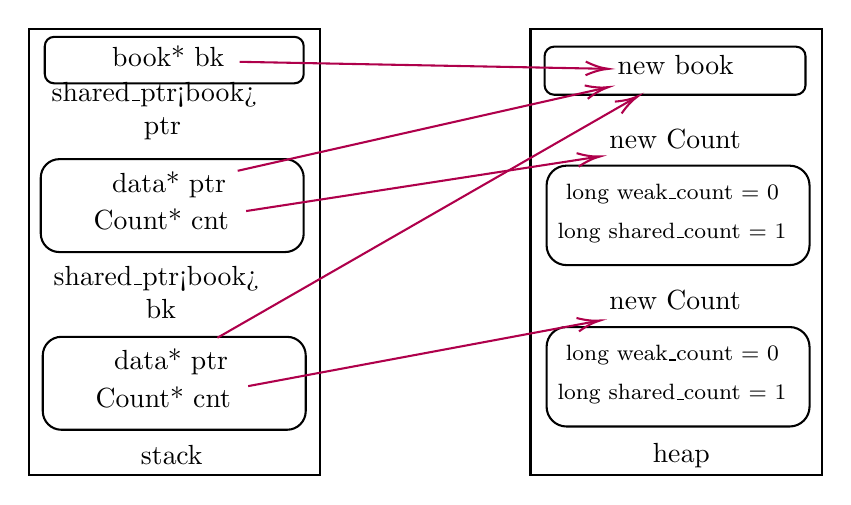
\begin{tikzpicture}[x=0.75pt,y=0.75pt,yscale=-1,xscale=1]
%uncomment if require: \path (0,300); %set diagram left start at 0, and has height of 300

%Rounded Rect [id:dp2187423114764504] 
\draw   (143.8,77.79) .. controls (143.8,72.85) and (147.81,68.84) .. (152.76,68.84) -- (261.54,68.84) .. controls (266.48,68.84) and (270.49,72.85) .. (270.49,77.79) -- (270.49,104.65) .. controls (270.49,109.6) and (266.48,113.61) .. (261.54,113.61) -- (152.76,113.61) .. controls (147.81,113.61) and (143.8,109.6) .. (143.8,104.65) -- cycle ;
%Shape: Rectangle [id:dp2941975065261839] 
\draw   (138,6) -- (278.23,6) -- (278.23,221.21) -- (138,221.21) -- cycle ;
%Shape: Rectangle [id:dp09704288189667065] 
\draw   (379.77,6) -- (520,6) -- (520,221.21) -- (379.77,221.21) -- cycle ;
%Rounded Rect [id:dp20297270277383261] 
\draw   (387.51,81.56) .. controls (387.51,76.27) and (391.8,71.98) .. (397.09,71.98) -- (504.61,71.98) .. controls (509.91,71.98) and (514.2,76.27) .. (514.2,81.56) -- (514.2,110.31) .. controls (514.2,115.6) and (509.91,119.89) .. (504.61,119.89) -- (397.09,119.89) .. controls (391.8,119.89) and (387.51,115.6) .. (387.51,110.31) -- cycle ;
%Rounded Rect [id:dp4729067946282406] 
\draw   (145.74,14.4) .. controls (145.74,11.93) and (147.74,9.93) .. (150.21,9.93) -- (266.01,9.93) .. controls (268.49,9.93) and (270.49,11.93) .. (270.49,14.4) -- (270.49,27.84) .. controls (270.49,30.31) and (268.49,32.31) .. (266.01,32.31) -- (150.21,32.31) .. controls (147.74,32.31) and (145.74,30.31) .. (145.74,27.84) -- cycle ;
%Rounded Rect [id:dp44562021942027163] 
\draw   (144.77,163.41) .. controls (144.77,158.46) and (148.78,154.45) .. (153.72,154.45) -- (262.5,154.45) .. controls (267.45,154.45) and (271.46,158.46) .. (271.46,163.41) -- (271.46,190.27) .. controls (271.46,195.21) and (267.45,199.22) .. (262.5,199.22) -- (153.72,199.22) .. controls (148.78,199.22) and (144.77,195.21) .. (144.77,190.27) -- cycle ;
%Rounded Rect [id:dp955530270440262] 
\draw   (387.51,159.32) .. controls (387.51,154.03) and (391.8,149.74) .. (397.09,149.74) -- (504.61,149.74) .. controls (509.91,149.74) and (514.2,154.03) .. (514.2,159.32) -- (514.2,188.07) .. controls (514.2,193.36) and (509.91,197.65) .. (504.61,197.65) -- (397.09,197.65) .. controls (391.8,197.65) and (387.51,193.36) .. (387.51,188.07) -- cycle ;
%Rounded Rect [id:dp3609920895859484] 
\draw   (386.54,19.27) .. controls (386.54,16.71) and (388.62,14.64) .. (391.18,14.64) -- (507.63,14.64) .. controls (510.19,14.64) and (512.26,16.71) .. (512.26,19.27) -- (512.26,33.18) .. controls (512.26,35.74) and (510.19,37.81) .. (507.63,37.81) -- (391.18,37.81) .. controls (388.62,37.81) and (386.54,35.74) .. (386.54,33.18) -- cycle ;

% Text Node
\draw (147.56,30.2) node [anchor=north west][inner sep=0.75pt]   [align=left] {shared\_ptr<book>\\ \ \ \ \ \ \ \ \ \ \ ptr};
% Text Node
\draw (176.68,73.3) node [anchor=north west][inner sep=0.75pt]   [align=left] {data* ptr};
% Text Node
\draw (167.76,91.36) node [anchor=north west][inner sep=0.75pt]   [align=left] {Count* cnt};
% Text Node
\draw (190.58,205.25) node [anchor=north west][inner sep=0.75pt]   [align=left] {stack};
% Text Node
\draw (437.22,204.47) node [anchor=north west][inner sep=0.75pt]   [align=left] {heap};
% Text Node
\draw (416.27,52.87) node [anchor=north west][inner sep=0.75pt]   [align=left] {new Count};
% Text Node
\draw (395.34,79.22) node [anchor=north west][inner sep=0.75pt]  [font=\footnotesize] [align=left] {long weak\_count = 0};
% Text Node
\draw (391.32,98.07) node [anchor=north west][inner sep=0.75pt]  [font=\footnotesize] [align=left] {long shared\_count = 1};
% Text Node
\draw (148.53,118.96) node [anchor=north west][inner sep=0.75pt]   [align=left] {shared\_ptr<book>\\ \ \ \ \ \ \ \ \ \ \ bk};
% Text Node
\draw (176.66,12.82) node [anchor=north west][inner sep=0.75pt]   [align=left] {book* bk};
% Text Node
\draw (177.65,158.91) node [anchor=north west][inner sep=0.75pt]   [align=left] {data* ptr};
% Text Node
\draw (168.73,176.98) node [anchor=north west][inner sep=0.75pt]   [align=left] {Count* cnt};
% Text Node
\draw (420.27,17.53) node [anchor=north west][inner sep=0.75pt]   [align=left] {new book};
% Text Node
\draw (416.27,130.63) node [anchor=north west][inner sep=0.75pt]   [align=left] {new Count};
% Text Node
\draw (395.34,156.98) node [anchor=north west][inner sep=0.75pt]  [font=\footnotesize] [align=left] {long weak\_count = 0};
% Text Node
\draw (391.32,175.83) node [anchor=north west][inner sep=0.75pt]  [font=\footnotesize] [align=left] {long shared\_count = 1};
% Connection
\draw [color={rgb, 255:red, 175; green, 0; blue, 75 }  ,draw opacity=1 ]   (239.66,21.95) -- (415.27,25.3) ;
\draw [shift={(417.27,25.34)}, rotate = 181.09] [color={rgb, 255:red, 175; green, 0; blue, 75 }  ,draw opacity=1 ][line width=0.75]    (10.93,-3.29) .. controls (6.95,-1.4) and (3.31,-0.3) .. (0,0) .. controls (3.31,0.3) and (6.95,1.4) .. (10.93,3.29)   ;
% Connection
\draw [color={rgb, 255:red, 175; green, 0; blue, 75 }  ,draw opacity=1 ]   (238.68,74.46) -- (415.32,34.59) ;
\draw [shift={(417.27,34.15)}, rotate = 167.28] [color={rgb, 255:red, 175; green, 0; blue, 75 }  ,draw opacity=1 ][line width=0.75]    (10.93,-3.29) .. controls (6.95,-1.4) and (3.31,-0.3) .. (0,0) .. controls (3.31,0.3) and (6.95,1.4) .. (10.93,3.29)   ;
% Connection
\draw [color={rgb, 255:red, 175; green, 0; blue, 75 }  ,draw opacity=1 ]   (228.91,154.91) -- (429.78,39.53) ;
\draw [shift={(431.51,38.53)}, rotate = 150.13] [color={rgb, 255:red, 175; green, 0; blue, 75 }  ,draw opacity=1 ][line width=0.75]    (10.93,-3.29) .. controls (6.95,-1.4) and (3.31,-0.3) .. (0,0) .. controls (3.31,0.3) and (6.95,1.4) .. (10.93,3.29)   ;
% Connection
\draw [color={rgb, 255:red, 175; green, 0; blue, 75 }  ,draw opacity=1 ]   (242.76,93.85) -- (411.29,67.85) ;
\draw [shift={(413.27,67.54)}, rotate = 171.23] [color={rgb, 255:red, 175; green, 0; blue, 75 }  ,draw opacity=1 ][line width=0.75]    (10.93,-3.29) .. controls (6.95,-1.4) and (3.31,-0.3) .. (0,0) .. controls (3.31,0.3) and (6.95,1.4) .. (10.93,3.29)   ;
% Connection
\draw [color={rgb, 255:red, 175; green, 0; blue, 75 }  ,draw opacity=1 ]   (243.73,178.2) -- (411.3,146.96) ;
\draw [shift={(413.27,146.59)}, rotate = 169.44] [color={rgb, 255:red, 175; green, 0; blue, 75 }  ,draw opacity=1 ][line width=0.75]    (10.93,-3.29) .. controls (6.95,-1.4) and (3.31,-0.3) .. (0,0) .. controls (3.31,0.3) and (6.95,1.4) .. (10.93,3.29)   ;

\end{tikzpicture}

\end{center}
		\item 这会释放两次资源, 因此事实上需要的返回操作是在对象内部返回定义在外部的智能指针, 一种实现方法
				是引入{\tt enable\_shared\_from\_this}
	\end{itemize}

\end{enumerate}
\subsubsection{\tt enable\_shared\_from\_this}
TODO:侵入式

一种容易想到的方法是在每一个需要返回对象智能指针的类中定义一个智能指针, 在构造一个\\{\tt shared\_ptr}的时候就
	需要初始化类中的这个智能指针, 基于前文, 这个指针应该为{\tt weak\_ptr}

更一般的, 让需要返回对象智能指针的类{\tt public}继承一个{\tt enable\_shared\_from\_this}, 
	在这个类中有一个{\tt weak\_ptr}用于进行上述相同的操作
\begin{lstlisting}
templte<class Tp> class enable_shared_from_this
private:	
	mutable weak_ptr<Tp> weak_this;
public:
	template <class Up> friend class shared_ptr;

    shared_ptr<Tp> shared_from_this() 
	{ return shared_ptr<Tp>(weak_this); }

struct book : enable_shared_from_this{
	void getshared(student* stu){
		stu->getnewbook(shared_from_this());
	}
};
\end{lstlisting}

而为了使用这个{\tt weak\_ptr}, 需要在构造这个对象的同时, 对其中的{\tt weak\_ptr}进行构造, 
	可能需要一个类似这样的构造版本
\begin{lstlisting}
explicit shared_ptr(Tp* p , bool need_shared = false) 
:ptr(p),cnt(new Counter) 
{ if(need_shared) p->weak_this=(*this); }//shared_ptr是enable_shared_from_this的友元
\end{lstlisting}

更一般的, 可以进行自动判断一个类是否继承了{\tt enable\_shared\_from\_this}, 若继承, 则自然有{\tt weak\_this}

上述代码就可更改为
\begin{lstlisting}
explicit shared_ptr(Ep* e) :ptr(e),cnt(new Counter) { enable_weak_this(e,e); }

template<class Up, class Ptr> 
enable_if_t<is_convertible_v<
	Ptr*, const enable_shared_from_this<Up>*
	>, /*SFINAE判断两种类型能否转换*/
void> enable_weak_this(const enable_shared_from_this<Up>* ep, Ptr* p) noexcept{
	using rawUp = remove_cv_t<Up>;
	if(ep && ep->weak_this.expired()){
		ep->weak_this = shared_ptr<rawUp>(
			*this, const_cast<rawUp*>(p)
		);
	} 
}//转换不成功则匹配下面这个版本, 接受任意参数, 不做任何行为	
void enable_weak_this(...) noexcept {}
\end{lstlisting}

文内代码见附录\space\nameref{appendix_code}\space\nameref{appendix_code_smart_ptr}

\subsection{\color{purple}{\tt noexcept}}
\label{cpp_c11_exception_safty}
参考{\tt effective c++}条款29
\subsubsection{基本异常安全保证}
如果异常抛出
\begin{enumerate}
	\item 程序内任何事物仍然保持在有效状态下, 没有任何对象或数据结构会因此而败坏
	\item 没有发生内存泄漏
	\item 不保证程序的前后状态不改变
\end{enumerate}

如使用智能指针代替裸指针
\subsubsection{强异常安全保证}
\begin{enumerate}
	\item 程序前后状态不改变
	\item 没有发生内存泄漏
\end{enumerate}

常见方法是{\tt copy and swap}, 对数据建一个副本, 将可能发生异常的操作使用这个副本, 
	成功后再将副本与原数据进行交换, 就能保证除非程序运行成功, 否则数据不会改变

根据具体场景选择合适的异常安全保证
\subsubsection{不抛掷异常保证}
在函数尾部添加{\tt noexcept}标识符, 承诺函数绝不抛出异常

{\tt noexcept}语义表达该函数应该不会抛出异常, \uline{让编译器不必多生成保护栈上对象安全析构的代码}

因此, 对于不抛掷异常保证函数一旦抛出异常就会立即终止进程而不再会被捕捉异常, 也可用于定位异常
\subsection{\color{purple}{\tt SFINAE}}
\href{https://zhuanlan.zhihu.com/p/338822185}{原文}

在{\tt C++}中针对不同参数类型做函数重载时, 编译器需要为一个调用选择一个最适合的函数,
	当这些重载函数包含模板函数时, 编译器一般会执行如下步骤
\begin{enumerate}
	\item 确定模板参数类型
	\item 将函数参数列表和返回值的模板参数替换掉{\tt (substitute)}
	\item 根据规则决定哪一个函数最匹配
	\item 但是替换的结果可能是毫无意义的. 这时, 编译器不会报错, 反而会忽略这个函数模板
\end{enumerate}

这个原则叫做{\tt: SFINAE(substitution failure is not an error)}

即使最终不需要被实例化的模板也要进行替换(不然就无法执行上面的第3步). 
	不过它只会替换直接出现在函数声明中的相关内容(不包含函数体)

\subsubsection{\tt enable\_if}
常见的{\tt SFINAE}实现方法, {\tt std::enable\_if<expr,type>}是一种类型萃取{\tt(type trait)}, 
	会根据给定的一个编译时期的表达式(第一个参数)来确定其行为
\begin{itemize}
	\item 如果这个表达式为{\tt true, std::enable\_if<>::type}会返回
	\begin{itemize}
		\item 如果没有第二个模板参数, 返回类型是{\tt void}
		\item 否则, 返回类型是其第二个参数的类型
	\end{itemize}
	\item 如果表达式结果{\tt false, std::enable\_if<>::type}不会被定义
		\\这会导致包含{\tt std::enable\_if<>}的模板被忽略掉
\end{itemize}
\begin{lstlisting}
template <bool, class Tp = void> struct enable_if {};
template <class Tp> struct enable_if<true, Tp> {typedef Tp type;};

template <bool Bp, class Tp = void> 
using enable_if_t = typename enable_if<Bp, Tp>::type;
\end{lstlisting}

通过这种方法可以实现类似这样的效果
\begin{lstlisting}
template<typename T, typename = enable_if_t<is_same_v<T,int>>>
void fun(T t) { cout<<1; }
//enable_if放在模板中只用于替换时类型判断, 不需要实际意义因此typename匿名
//或者
template<typename T>
enable_if_t<is_same_v<T,int>> fun(T t) { cout<<1; }
//模板替换成功后enable_if正好返回void

void fun(...) { cout<<2; }
\end{lstlisting}
当传入参数是{\tt int}类型时, {\tt enable\_if}才有成员{\tt type}的定义, 否则函数模板会被忽略, 从而匹配另一个重载函数
\subsection{\color{purple}{函数}}
\subsubsection{函数指针}
函数指针与函数的区别
\begin{enumerate}
	\item 函数指针本身存储在内存中的栈或堆中, 指向的函数存储在代码段中
	\item 函数指针是一个变量, 而函数本身不是变量, 它是一个代码段
	\item 函数指针可以作为函数参数、返回值或者变量使用, 而函数只能作为函数调用时使用
	\item 函数指针可以动态地指向不同的函数, 而函数则固定指向特定的代码段
	\item 函数指针可以通过函数指针的赋值修改它所指向的函数, 而函数本身不支持这种操作
\end{enumerate}

函数在以下情况下会变成函数指针
\begin{enumerate}
	\item 当函数名作为参数传递给另一个函数时, 函数名会自动转换为函数指针
	\item 当函数指针被赋值为函数名时, 函数名会自动转换为函数指针
	\item 当函数指针作为返回值返回时, 返回的是函数指针而不是函数本身
\end{enumerate}

\subsubsection{仿函数}
\columnratio{0.5}
\begin{paracol}{2}
	\begin{leftcolumn}
		\begin{lstlisting}
struct test{
	test(int c):c(c){}
	int c;
	void operator()(int a,int b){
		cout<<a+b+c;
	}
};
int main(){
	int a=1,b=2,c=3;
	test t(c);
	t(a,b);
}
			\end{lstlisting}
	\end{leftcolumn}
	\begin{rightcolumn}
		通过在结构体中重载()运算符可以使一个结构体对象像函数那样去工作, 
			类外其它数据传递可以通过构造函数的方式去捕获而不是全部通过参数传递.
	\end{rightcolumn}
\end{paracol}

\subsubsection{{\tt lambda}}
{\tt lambda}也叫匿名仿函数, 通过一种特殊的语法规则能够简化仿函数的使用

一个完整的{\tt lambda}示例
\begin{lstlisting}
[capture] (input_type para) option -> return_type { function body; };
[capture] (input_type para) \*     可省略       *\ { function body; };
\end{lstlisting}
这样一个{\tt lambda}函数本身是一个右值, 可以将其传递给一个左值, 或者直接调用
\begin{lstlisting}
auto f = [capture] (input_type para) option -> return_type { function body; };

[](int a){cout<<a;}(1);
\end{lstlisting}

实际上它等同于这样一个仿函数

\begin{lstlisting}
struct lambda_random_label{
	lambda_random_label(capture):capture{}
	return_type operator()(input_type para){
		function body;
	}
};
lambda_random_label f = [capture] (input_type para) { function body; };
//f就是这个匿名的lambda结构体的一个实例
\end{lstlisting}

其中{\tt capture}分为按值捕获{\tt[\&]}和按引用捕获{\tt[=]}, 区别在于函数体内能否改变外部的值

{\tt lambda}中的{\tt option}可以写{\tt mutable}或者不填, 几种可能的实现
\begin{enumerate}
	\item 如果不填则仿函数重载运算符是默认{\tt const}函数, 此时无法更改捕获列表中按值捕获的值
	\item 如果不填则默认按值捕获的成员为{\tt const}类型
	\item 仿函数重载运算符是{\tt const}函数, 通过给成员加上{\tt mutable}使其可修改
\end{enumerate}

{\tt lambda}函数能够自动推断返回值类别, 一般情况下不需要添加尾返回类型, 除非返回值存在需要类型转换的情况, 
	如同时存在返回{\tt int}和{\tt bool}的情况需要指明返回{\tt int}还是{\tt bool}, 即使在明确指明{\tt lambda}
	的类型是一个具体的{\tt function<()>}情况下依旧会面临这个问题, 因为是先有的{\tt lambda}, 将其赋给{\tt function<()>},而不是{\tt lambda}
	本身就是这样一个类型, 其返回类型还是要自动判断或者尾返回类型指定

如果需要递归调用, 除了参数列表中传递{\tt self}的方法, 可以将{\tt lambda}赋给一个显式类型{\tt function}, 并捕获自身
\subsubsection{{\tt function}}
对于{\tt C++}中几种可调用对象, 如函数、函数指针、仿函数、{\tt lambda}等

虽然它们可能使用方式相同即接收参数类型相同,返回值类型也相同, 但事实上是完全不同的对象类型, 
	函数和函数指针都可以当作函数指针类型使用, 而仿函数和lambda是一个类类型

如果想把这些看似一样的函数对象放在一起就会遇到问题
\begin{lstlisting}
int f1(int i,int j){return i+j;}
auto f2 = [](int i,int j){return i+j;};
vector<int(*)(int,int)> funv;
funv.emplace_back(f1);
funv.emplace_back(f2);//error lambda不是函数指针
\end{lstlisting}

通过{\tt function<()>}可以将所有的函数对象转换成相同的类型
\begin{lstlisting}
int f1(int i,int j){return i+j;}
auto f2 = [](int i,int j){return i+j;};
int (*f3)(int,int) = f1;
vector<function<int(int,int)>> funv;
funv.emplace_back(f1);
funv.emplace_back(f2);
funv.emplace_back(f3);
\end{lstlisting}

对于函数重载时, {\tt function<()>}无法判别两个同名函数究竟是传入谁, {\tt function<()>}自身指明的类型不会
	用于对传入的函数对象类型进行判断和修饰, 根据函数重载的规则, 编译器自身也无法在没有传参的情况下就判断调用的函数版本
\begin{lstlisting}
	int f(int i,int j){return i+j;}
	int f(int i      ){return i;}
	
	function<int(int)> fun = f;//error <overloaded function type>

	int (*fp)(int) = f;
	function<int(int)> fun = fp;//     <int (*)(int)>
\end{lstlisting}

可行方法是用函数指针指明是哪一个重载

